\documentclass[12pt,a4paper,oneside]{report}

\usepackage[utf8]{inputenc}
\usepackage[T1]{fontenc}
\usepackage{mathptmx}
\usepackage{geometry}
\geometry{
    a4paper,
    top=25mm,
    bottom=25mm,
    left=35mm,
    right=20mm,
    headheight=14pt
}

\usepackage{amsmath,amssymb,amsfonts}
\usepackage{graphicx}
\graphicspath{{../../figures/}{../figures/}{./figures/}{figures/}}
\usepackage{booktabs}
\usepackage{longtable}
\usepackage{array}
\usepackage{float}
\usepackage{setspace}
\onehalfspacing

\usepackage{fancyhdr}
\pagestyle{fancy}
\fancyhf{}
\fancyhead[L]{\slshape \small Project I -- Newton--Raphson AC Power Flow Analysis}
\fancyhead[R]{\slshape \small HUST -- SEEE}
\fancyfoot[C]{\thepage}
\renewcommand{\headrulewidth}{0.4pt}
\renewcommand{\footrulewidth}{0pt}

\usepackage{titlesec}
\titleformat{\chapter}[hang]{\bfseries\Large}{\thechapter.\ }{0pt}{}
\titlespacing*{\chapter}{0pt}{-10pt}{15pt}
\titleformat{\section}[hang]{\bfseries\large}{\thesection\ }{0pt}{}
\titleformat{\subsection}[hang]{\bfseries\normalsize}{\thesubsection\ }{0pt}{}

\usepackage{tocloft}
\renewcommand{\cftchapleader}{\cftdotfill{\cftdotsep}}

\usepackage{xcolor}
\usepackage{hyperref}
\hypersetup{
    colorlinks=true,
    linkcolor=black,
    citecolor=black,
    urlcolor=blue
}

\begin{document}

% ==================== COVER PAGE (100% ENGLISH) ====================
\begin{titlepage}
\begin{center}
    {\large \textbf{HANOI UNIVERSITY OF SCIENCE AND TECHNOLOGY}}\\[4pt]
    {\large \textbf{SCHOOL OF ELECTRICAL AND ELECTRONIC ENGINEERING}}\\[4pt]
    {\large \textbf{DEPARTMENT OF POWER SYSTEMS}}\\[35pt]

    
\includegraphics[width=36mm]{../figures/hust_emblem.png}\\[40pt]

    {\Large \textbf{PROJECT I REPORT}}\\[12pt]
    {\large \textbf{COURSE CODE: EE3810E}}\\[25pt]

    {\LARGE \textbf{AC POWER FLOW ANALYSIS USING NEWTON--RAPHSON METHOD: MATHEMATICAL FORMULATION, STEP-BY-STEP NUMERICAL VERIFICATION, AND SOFTWARE CROSS-VALIDATION}}\\[45pt]

    \begin{tabular}{ll}
        \textbf{Author / Student:} & \textbf{La Huy Gia Huy} \\
        \textbf{Student ID:} & \textbf{202412885} \\
        \textbf{Class / Cohort:} & \textbf{EE - E18} \\
        \textbf{Academic Program:} & Power Systems and Renewable Energy - 02 \\
        \textbf{Degree Track:} & Elite Engineering Education Program \\
        \textbf{Email:} & Huy.lhg2412885@sis.hust.edu.vn \\[14pt]
        \textbf{Academic Supervisor:} & \textbf{Dr. Nguyen Hoang Viet} \\
        \textbf{Department:} & Power Systems Department, SEEE \\
        \textbf{Institution:} & Hanoi University of Science and Technology \\
    \end{tabular}

    \vfill
    {\large \textbf{HANOI, ACADEMIC YEAR 2026--2027}}
\end{center}
\end{titlepage}



% ==================== PRELIMINARY PAGES (100% ENGLISH) ====================
\pagenumbering{roman}

% --- PROJECT ASSIGNMENT SHEET ---
\chapter*{Project Assignment Sheet}
\addcontentsline{toc}{chapter}{Project Assignment Sheet}

\begin{spacing}{1.15}
\begin{enumerate}\setlength{\itemsep}{1.5pt}\setlength{\parskip}{0pt}
    \item \textbf{Student Information:}
    \begin{itemize}\setlength{\itemsep}{0.5pt}\setlength{\parskip}{0pt}
        \item Full Name: \textbf{La Huy Gia Huy} \quad Student ID: \textbf{202412885}
        \item Cohort / Class: EE - E18 \quad Degree Program: Power Systems and Renewable Energy - 02
        \item School: School of Electrical and Electronic Engineering (SEEE), HUST
    \end{itemize}
    \item \textbf{Official Project Title:}
    \begin{itemize}\setlength{\itemsep}{0.5pt}\setlength{\parskip}{0pt}
        \item \textit{"AC Power Flow Analysis using Newton--Raphson Method: Mathematical Formulation, Step-by-Step Numerical Verification, and Software Cross-Validation"}
    \end{itemize}
    \item \textbf{Engineering Objectives and Scope of Work:}
    \begin{itemize}\setlength{\itemsep}{0.5pt}\setlength{\parskip}{0pt}
        \item Formulate continuous mathematical physics of AC power flow in polar coordinates, assembling nodal admittance matrix ($\mathbf{Y}_{\text{bus}}$) and deriving analytical closed-form equations for all eight entries of Jacobian matrix ($\mathbf{H}, \mathbf{N}, \mathbf{M}, \mathbf{L}$).
        \item Execute white-box, step-by-step manual numerical benchmark calculation on a 3-bus transmission network for Iteration 1 ($m = 0 \to 1$), documenting every numerical substitution and matrix operation.
        \item Conduct multi-tier cross-validation between manual calculations and numerical solver to IEEE-754 double precision ($< 10^{-16}\text{ p.u.}$), verifying quadratic convergence down to $\varepsilon = 10^{-10}\text{ p.u.}$ across 4 iterations, and proving active/reactive energy conservation.
        \item Investigate grid physical behavior across four core operational scenarios: load scaling (80\%--120\%), generator voltage regulation, shunt capacitive compensation, and $N-1$ line outage contingencies.
    \end{itemize}
    \item \textbf{Project Milestones and Timeline:}
    \begin{itemize}\setlength{\itemsep}{0.5pt}\setlength{\parskip}{0pt}
        \item Weeks 1--4: Literature review, network mathematical modeling, and per-unit normalization.
        \item Weeks 5--8: Closed-form Jacobian derivation, algorithm design, and flowcharts.
        \item Weeks 9--12: Step-by-step numerical benchmark calculation and solver cross-validation.
        \item Weeks 13--16: Operational scenario analysis, engineering report compilation, and final review.
    \end{itemize}
\end{enumerate}

\vspace{18pt}
\noindent
\begin{minipage}[t]{0.48\textwidth}
    \centering
    \textbf{Head of Department}\\[35pt]
    \textbf{Assoc. Prof. Dr. Nguyen Duc Huy}
\end{minipage}
\hfill
\begin{minipage}[t]{0.48\textwidth}
    \centering
    \textbf{Academic Supervisor}\\[35pt]
    \textbf{Dr. Nguyen Hoang Viet}
\end{minipage}
\end{spacing}

\clearpage

% --- DECLARATION OF ACADEMIC INTEGRITY ---
\chapter*{Declaration of Academic Integrity}
\addcontentsline{toc}{chapter}{Declaration of Academic Integrity}

I hereby declare that this Project I report entitled \textit{"AC Power Flow Analysis using Newton--Raphson Method: Mathematical Formulation, Step-by-Step Numerical Verification, and Software Cross-Validation"} is the authentic and original outcome of my independent research, mathematical derivation, and computational validation conducted under the supervision of \textbf{Dr. Nguyen Hoang Viet} at the Department of Power Systems, School of Electrical and Electronic Engineering (SEEE), Hanoi University of Science and Technology (HUST).

All mathematical formulations, nodal admittance matrix assembly procedures, closed-form Jacobian derivations, manual benchmark calculations, and operational scenario assessments presented in this report were conducted and verified by myself. All scientific literature, foundational textbook formulas, and technical publications have been fully cited and acknowledged in strict accordance with the academic integrity regulations and ethical standards of Hanoi University of Science and Technology.

\vspace{45pt}
\begin{flushright}
    \textbf{Author}\\[45pt]
    \textbf{La Huy Gia Huy}\\
    Student ID: 202412885\\
    Cohort: EE - E18, SEEE, HUST
\end{flushright}

\clearpage

% --- ACKNOWLEDGEMENTS ---
\chapter*{Acknowledgements}
\addcontentsline{toc}{chapter}{Acknowledgements}

First and foremost, I wish to express my deepest gratitude and sincere appreciation to my academic supervisor, \textbf{Dr. Nguyen Hoang Viet}, for his invaluable pedagogical guidance, technical insights, and continuous encouragement throughout the conception, mathematical verification, and software development of this Project I. His rigorous standards in power system modeling and scientific research have profoundly shaped the precision and thoroughness of this work.

I would also like to extend my sincere gratitude to all the esteemed faculty members and lecturers of the Department of Power Systems and the School of Electrical and Electronic Engineering (SEEE) at Hanoi University of Science and Technology. The curriculum of the Elite Engineering Program EE-E18 in Power Systems and Renewable Energy has equipped me with the solid theoretical foundation in electrical network analysis, numerical computation, and grid modeling necessary to execute this project successfully.

Finally, I convey my heartfelt thanks to my family, colleagues, and classmates in EE-E18 for their continuous encouragement, technical discussions, and steadfast moral support throughout my academic studies at HUST.

\vspace{35pt}
\begin{flushright}
    Hanoi, October 2026\\
    \textit{La Huy Gia Huy}
\end{flushright}

\clearpage

% --- EXECUTIVE SUMMARY / ABSTRACT ---
\chapter*{Executive Summary}
\addcontentsline{toc}{chapter}{Executive Summary}

Steady-state alternating current (AC) power flow analysis is the foundational mathematical technique underpinning power systems engineering, serving as the prerequisite for operational security dispatch, expansion planning, voltage stability assessment, and contingency analysis. In power engineering practice and education, commercial software packages frequently operate as black boxes, concealing the underlying non-linear equation formulation, matrix structure, analytical partial derivatives, and numerical convergence characteristics.

This Project I report presents a comprehensive, white-box, three-tier engineering methodology for AC power flow analysis based on the Polar Newton--Raphson algorithm:
\begin{itemize}
    \item \textbf{Tier 1 (Rigorous Analytical Formulation):} The non-linear AC power flow equations are derived from first physical principles and Kirchhoff's Current Law, culminating in the closed-form analytical derivation of all eight elements of the four-block partitioned Jacobian matrix ($\mathbf{H}, \mathbf{N}, \mathbf{M}, \mathbf{L}$), eliminating numerical finite-difference errors.
    \item \textbf{Tier 2 (Transparent Manual Benchmark):} An exhaustive, step-by-step manual numerical benchmark calculation is executed on an IEEE-based 3-bus transmission test network for Iteration 1 ($m = 0 \to 1$), documenting every primitive admittance, matrix assembly, trigonometric evaluation, power mismatch, Jacobian coefficient, and matrix inversion without skipping intermediate steps.
    \item \textbf{Tier 3 (Multi-Tier Cross-Validation and Physical Analysis):} The manual benchmark is cross-validated against the developed numerical solver down to IEEE-754 double precision ($< 10^{-16}\text{ p.u.}$ discrepancy), confirming the theoretical quadratic convergence rate down to a tolerance of $\varepsilon = 10^{-10}\text{ p.u.}$ across 4 iterations and establishing global active and reactive power balance. Finally, grid physical mechanics are investigated across four operational scenarios: system load scaling (80\% to 120\%), generator voltage regulation, shunt capacitor compensation, and $N-1$ line outage contingencies.
\end{itemize}

\vspace{15pt}
\noindent \textbf{Keywords:} AC Power Flow, Polar Newton--Raphson Method, Nodal Admittance Matrix ($\mathbf{Y}_{\text{bus}}$), Analytical Jacobian Matrix, Step-by-Step Numerical Verification, Software Cross-Validation, $N-1$ Contingency Screening, Power Systems Engineering.

\clearpage

% --- NOMENCLATURE & ABBREVIATIONS ---
\chapter*{Nomenclature and Abbreviations}
\addcontentsline{toc}{chapter}{Nomenclature and Abbreviations}

\section*{List of Abbreviations}
\begin{longtable}{ll}
\toprule
\textbf{Abbreviation} & \textbf{Full Engineering Description} \\
\midrule
AC & Alternating Current \\
AVR & Automatic Voltage Regulator \\
EMS & Energy Management System \\
HUST & Hanoi University of Science and Technology \\
IEEE & Institute of Electrical and Electronics Engineers \\
KCL & Kirchhoff's Current Law \\
KVL & Kirchhoff's Voltage Law \\
NR & Newton--Raphson Method \\
OPF & Optimal Power Flow \\
OLTC & On-Load Tap Changer \\
p.u. & Per-Unit Normalization System \\
PQ & Load Bus (Active and Reactive Power Specified) \\
PV & Voltage-Controlled Bus (Active Power and Voltage Magnitude Specified) \\
SEEE & School of Electrical and Electronic Engineering \\
Slack & Swing / Reference Bus (Voltage Magnitude and Phase Angle Specified) \\
SLD & Single-Line Diagram \\
TSO & Transmission System Operator \\
ZIP & Constant Impedance (Z), Constant Current (I), Constant Power (P) Load Model \\
\bottomrule
\end{longtable}

\section*{List of Mathematical Symbols}
\begin{longtable}{ll}
\toprule
\textbf{Symbol} & \textbf{Physical Meaning / Engineering Definition} \\
\midrule
$S_{\text{base}}$ & Three-phase system base apparent power ($100.0\text{ MVA}$) \\
$U_{\text{base}}$ & Line-to-line base RMS voltage ($\text{kV}$) \\
$Z_{\text{base}}$ & Base impedance ($\Omega$), defined as $U_{\text{base}}^2 / S_{\text{base}}$ \\
$I_{\text{base}}$ & Base line current ($\text{kA}$), defined as $S_{\text{base}} / (\sqrt{3} U_{\text{base}})$ \\
$N$ & Total number of buses in the electrical transmission grid \\
$N_{\text{PV}}$ & Number of voltage-controlled (PV) generator buses \\
$N_{\text{PQ}}$ & Number of uncontrolled load (PQ) buses \\
$U_i, \vert{}U_i\vert{}$ & Bus voltage magnitude at bus $i$ ($\text{p.u.}$) \\
$\delta_i$ & Bus voltage phase angle at bus $i$ ($\text{rad}$ or degrees) \\
$\delta_{ij}$ & Phase angle difference between bus $i$ and bus $j$, $\delta_i - \delta_j$ ($\text{rad}$) \\
$P_i^{\text{calc}}, Q_i^{\text{calc}}$ & Calculated active and reactive power injections at bus $i$ ($\text{p.u.}$) \\
$P_i^{\text{sch}}, Q_i^{\text{sch}}$ & Scheduled net active and reactive power injections ($P_{Gi} - P_{Di}, Q_{Gi} - Q_{Di}$) \\
$\Delta P_i, \Delta Q_i$ & Active and reactive power mismatches at bus $i$ ($\text{p.u.}$) \\
$\mathbf{Y}_{\text{bus}}$ & Complex $N \times N$ nodal admittance matrix, $\mathbf{Y}_{\text{bus}} = \mathbf{G} + j\mathbf{B}$ \\
$Y_{ij}, \vert{}Y_{ij}\vert{}\angle\theta_{ij}$ & Mutual admittance between bus $i$ and bus $j$ ($G_{ij} + jB_{ij}$) \\
$Y_{ii}$ & Self-admittance of bus $i$ ($G_{ii} + jB_{ii}$) \\
$z_{ij}$ & Branch series impedance, $z_{ij} = r_{ij} + jx_{ij}$ ($\text{p.u.}$) \\
$y_{ij}$ & Branch series admittance, $y_{ij} = z_{ij}^{-1} = g_{ij} + jb_{ij}$ ($\text{p.u.}$) \\
$b_{ij0}$ & Half-line charging capacitive susceptance, $b_{ij0} = B_{ij}/2$ ($\text{p.u.}$) \\
$\mathbf{J}$ & Polar Newton--Raphson Jacobian matrix, partitioned into $\mathbf{H}, \mathbf{N}, \mathbf{M}, \mathbf{L}$ \\
$\mathbf{H}$ & Jacobian sub-matrix block: $\partial \mathbf{P} / \partial \boldsymbol{\delta}$ \\
$\mathbf{N}$ & Jacobian sub-matrix block: $\partial \mathbf{P} / \partial \mathbf{U}$ \\
$\mathbf{M}$ & Jacobian sub-matrix block: $\partial \mathbf{Q} / \partial \boldsymbol{\delta}$ \\
$\mathbf{L}$ & Jacobian sub-matrix block: $\partial \mathbf{Q} / \partial \mathbf{U}$ \\
$\Delta \mathbf{x}^{(m)}$ & Iterative state correction vector, $[\Delta \boldsymbol{\delta}^{(m)}, \Delta \mathbf{U}^{(m)}]^T$ \\
$m$ & Iteration counter ($m = 0, 1, 2, \dots$) \\
$\varepsilon$ & Convergence stopping tolerance threshold ($10^{-10}\text{ p.u.}$) \\
$P_{ij}, Q_{ij}$ & Active and reactive power flows from bus $i$ toward bus $j$ ($\text{MW, Mvar}$) \\
$\Delta P_{ij}, \Delta Q_{ij}$ & Active power loss and reactive power absorption along branch $i-j$ \\
$\Delta P_{\Sigma}, \Delta Q_{\Sigma}$ & System-wide total active and reactive power transmission losses \\
\bottomrule
\end{longtable}

\clearpage

% --- TABLE OF CONTENTS & LISTS ---
\tableofcontents
\clearpage
\listoftables
\clearpage
\listoffigures
\clearpage

% ==================== MAIN REPORT CHAPTERS ====================
\pagenumbering{arabic}

% ----------------------------------------------------
% CHAPTER 1: INTRODUCTION
% ----------------------------------------------------
\chapter{Introduction}

\section{Fundamental Role of Steady-State AC Power Flow in Power Grid Engineering}
The electric power transmission grid is one of the most critical and expansive engineering systems in modern society. Its primary operational requirement is the continuous, instantaneous, and stable equilibrium between electrical energy generation and dynamic consumer demand, subject to physical transmission laws and statutory operating constraints. In the hierarchy of power system analytics, steady-state alternating current (AC) power flow analysis---traditionally referred to as load flow analysis---forms the mathematical bedrock upon which power system planning, operational scheduling, and real-time security control depend.

Under balanced three-phase sinusoidal steady-state operation at nominal fundamental frequency ($50\text{ Hz}$ or $60\text{ Hz}$), the dynamic differential equations describing synchronous generators, rotating machines, transmission line electromagnetic waves, and network transients reduce to a set of non-linear algebraic equations. Power flow analysis determines the steady-state operating state of the electrical network, defined by the nodal voltage magnitude vector $\mathbf{U} = [U_1, U_2, \dots, U_N]^T$ and phase angle vector $\boldsymbol{\delta} = [\delta_1, \delta_2, \dots, \delta_N]^T$. Once this nodal state vector is resolved, all secondary operating quantities across the power system can be directly evaluated via analytical post-processing:
\begin{enumerate}
    \item \textbf{Directional Branch Power Flows:} Real power ($P_{ij}$) and reactive power ($Q_{ij}$) transferred through every transmission line and transformer corridor.
    \item \textbf{Network Power Losses:} Active power dissipation ($\Delta P_{ij} = I_{ij}^2 r_{ij}$) and reactive power absorption or generation ($\Delta Q_{ij} = I_{ij}^2 x_{ij} - U_i^2 b_{ij0}$) across the system.
    \item \textbf{Generator Duties:} Total active and reactive power supplied by the slack generator ($P_{G1}, Q_{G1}$) and the reactive power duties ($Q_{Gk}$) required from all voltage-controlled generators.
    \item \textbf{Voltage Quality and Security Assessment:} Verification of whether bus voltage profiles satisfy statutory operating limits (typically $0.95\text{ p.u.} \le U_i \le 1.05\text{ p.u.}$).
\end{enumerate}

Power flow analysis is indispensable across several operational and planning domains:
\begin{itemize}
    \item \textbf{Long-Term Expansion Planning:} Power system engineers simulate multi-year load growth scenarios (over 5 to 20-year horizons) to identify transmission line bottlenecks, evaluate transformer overloading, and determine the optimal allocation of reactive power compensation (e.g., shunt capacitors, SVCs, STATCOMs).
    \item \textbf{Optimal Power Flow (OPF) and Economic Dispatch:} In energy management systems (EMS), power flow equations serve as the physical network equality constraints within which generation dispatch algorithms minimize operating costs or carbon emissions while respecting thermal line ratings and voltage limits.
    \item \textbf{Operational Security and $N-1$ Contingency Screening:} Transmission system operators (TSOs) routinely execute thousands of automated power flow calculations every few minutes to verify $N-1$ grid security. This screening evaluates whether the unexpected loss of any critical component (e.g., an overhead transmission line, large generator, or autotransformer) causes cascading line overloads or voltage instability.
\end{itemize}

\section{Research Objectives and Scope of Work}
While commercial power systems software suites (such as PSS/E, DIgSILENT PowerFactory, ETAP, and PowerWorld) automate power flow calculations, their closed proprietary nature often conceals key mathematical and algorithmic mechanisms. Numerical challenges such as Jacobian ill-conditioning, near-singular derivative matrices, flat-start convergence dynamics, and generator reactive capability limit violations are frequently hidden from view.

The primary objective of this project is to develop an uncompromised, mathematically transparent, white-box investigation of the AC power flow problem utilizing the Polar Newton--Raphson iterative algorithm. The specific technical scope includes:
\begin{enumerate}
    \item \textbf{Rigorous Mathematical Formulation:} Deriving the AC power flow equations from first principles of complex circuit theory and Kirchhoff's Current Law (KCL), culminating in explicit polar equations and closed-form analytical derivations of all eight entries of the four-block partitioned Jacobian matrix.
    \item \textbf{Step-by-Step Manual Numerical Benchmark:} Providing a complete, fully documented manual calculation on an IEEE-based 3-bus transmission network for Iteration 1 ($m = 0 \to 1$). Every numerical substitution---primitive branch admittances, nodal admittance matrix construction, power mismatch calculation, Jacobian sub-matrix evaluation, and linear matrix inversion---is detailed explicitly without skipping intermediate steps.
    \item \textbf{Machine-Precision Software Cross-Validation:} Performing direct 1:1 cross-validation between the manual derivations and the output of the developed numerical solver to IEEE-754 double precision, verifying the quadratic convergence trajectory down to $\varepsilon = 10^{-10}\text{ p.u.}$ across 4 iterations, and confirming global active and reactive power balance.
    \item \textbf{Physical Operational Scenario Testing:} Assessing network behavior under four operational stress conditions:
    \begin{itemize}
        \item \textit{System Load Scaling (80\% to 120\%):} Evaluating longitudinal line voltage drop and quadratic loss growth.
        \item \textit{Generator Terminal Voltage Regulation:} Examining reactive power injection shifts and voltage support at load buses.
        \item \textit{Shunt Capacitive Compensation:} Quantifying reactive current reduction, voltage profile elevation, and transmission loss reduction.
        \item \textit{$N-1$ Transmission Line Outages:} Analyzing topological line disconnections, line loading redistribution, bus phase angle separation, and voltage collapse proximity.
    \end{itemize}
\end{enumerate}

\section{Three-Tier Verification-Driven Engineering Methodology}
To ensure academic rigor, this study avoids heuristic approximations and black-box abstractions. We implement a structured \textbf{3-Tier Research Engineering Workflow}:
\begin{itemize}
    \item \textbf{Tier 1 (Analytical Formulation):} Derives the continuous mathematical equations of the AC transmission grid, establishing coordinate systems, base value normalizations, sign conventions, and non-linear partial derivatives without numerical discretization errors.
    \item \textbf{Tier 2 (White-Box Numerical Benchmark):} Translates the continuous formulation into an exact discrete numerical step for Iteration 1 ($m = 0 \to 1$). Every numerical substitution is performed transparently, establishing an indisputable baseline for algorithm verification.
    \item \textbf{Tier 3 (Multi-Tier Cross-Validation and Operational Analysis):} Cross-validates the developed numerical solver against the manual baseline, tracks quadratic convergence down to $10^{-16}\text{ p.u.}$ machine noise, conducts global system power audits, and interprets physical power system behavior under operational constraints.
\end{itemize}

\section{Structural Organization of the Report}
The remainder of this report is organized into five comprehensive chapters:
\begin{itemize}
    \item \textbf{Chapter 2 (Power System Modeling \& Network Topology):} Formulates physical component models, per-unit base scaling, nominal $\pi$-equivalent circuits of transmission lines and off-nominal transformers, systematic bus classification (Slack, PV, PQ), static ZIP load models, and the algorithmic synthesis of the nodal admittance matrix ($\mathbf{Y}_{\text{bus}}$).
    \item \textbf{Chapter 3 (Mathematical Formulation \& Newton--Raphson Solver):} Derives the non-linear polar AC power flow equations, multidimensional Taylor series linearization, closed-form analytical derivations of all eight entries of the four-block Jacobian matrix ($\mathbf{H}, \mathbf{N}, \mathbf{M}, \mathbf{L}$), stopping criteria, and post-convergence branch flow and loss formulations.
    \item \textbf{Chapter 4 (Numerical Verification \& Exhaustive Test Scenarios):} Details the complete manual benchmark calculation on the 3-bus network for Iteration 1, tabulates direct 1:1 cross-validation against the developed numerical solver, traces the quadratic convergence profile, verifies global power balance, and analyzes four operational grid scenarios.
    \item \textbf{Chapter 5 (Conclusion \& Engineering Insights):} Synthesizes theoretical and numerical findings, reflects on Newton--Raphson algorithmic characteristics, and outlines future research directions in computational power systems.
\end{itemize}

% ----------------------------------------------------
% CHAPTER 2: POWER SYSTEM MODELING & NETWORK TOPOLOGY
% ----------------------------------------------------
\chapter{Power System Modeling \& Network Topology}

\section{Per-Unit (p.u.) Normalization System and Base Scaling Laws}
In modern interconnected power systems, electrical power is generated at medium voltage ($10.5\text{ kV} - 24\text{ kV}$), stepped up to extra-high voltage (EHV: $220\text{ kV} - 500\text{ kV}$) for bulk transmission over long distances, stepped down to sub-transmission levels ($110\text{ kV}$), and distributed through medium-voltage ($22\text{ kV}$) and low-voltage ($0.4\text{ kV}$) networks. Direct calculation of voltages, currents, and impedances in physical physical units (V, A, $\Omega$) across multi-voltage networks requires carrying ideal transformer voltage ratios ($N_1 : N_2$) through every network loop and node.

To eliminate transformer ideal transformation ratios, improve numerical matrix conditioning, and provide an intuitive scale for evaluating equipment loadings, the \textbf{Per-Unit (p.u.) system} is universally adopted:
\begin{equation}
\text{Value in per-unit (p.u.)} = \frac{\text{Actual Value in Physical Units}}{\text{Base Value in Physical Units}}
\end{equation}

\subsection{Base Quantities Selection and Derivation}
For an entire interconnected AC power grid, two independent base quantities are arbitrarily chosen to establish system-wide scaling:
\begin{enumerate}
    \item \textbf{System Three-Phase Apparent Power Base ($S_{\text{base}}$):} Selected as a round decimal number, conventionally $S_{\text{base}} = 100.0\text{ MVA}$ across transmission network studies. This value remains constant across all voltage levels throughout the entire system.
    \item \textbf{Line-to-Line Voltage Base ($U_{\text{base}}$):} Chosen for each voltage zone equal to the nominal operating line-to-line RMS voltage of that specific network section (e.g., $U_{\text{base}} = 500\text{ kV}, 220\text{ kV}, 110\text{ kV}$).
\end{enumerate}

Once $S_{\text{base}}$ (three-phase) and $U_{\text{base}}$ (line-to-line) are designated for a network zone, all dependent base parameters---base current ($I_{\text{base}}$), base impedance ($Z_{\text{base}}$), and base admittance ($Y_{\text{base}}$)---are derived from balanced three-phase circuit relations:
\begin{equation}
I_{\text{base}} = \frac{S_{\text{base}}}{\sqrt{3} U_{\text{base}}} \quad [\text{kA}]
\end{equation}
\begin{equation}
Z_{\text{base}} = \frac{U_{\text{base}} / \sqrt{3}}{I_{\text{base}}} = \frac{U_{\text{base}}^2}{S_{\text{base}}} \quad [\Omega]
\end{equation}
\begin{equation}
Y_{\text{base}} = \frac{1}{Z_{\text{base}}} = \frac{S_{\text{base}}}{U_{\text{base}}^2} \quad [\text{S} \text{ or } \Omega^{-1}]
\end{equation}
where $S_{\text{base}}$ is in $\text{MVA}$, $U_{\text{base}}$ in $\text{kV}$, $Z_{\text{base}}$ in $\Omega$, and $I_{\text{base}}$ in $\text{kA}$.

\subsection{Single-Phase vs. Three-Phase Consistency}
A major mathematical advantage of the per-unit system is that three-phase power equations and single-phase circuit equations become mathematically identical. Consider the total three-phase complex power $S_{\text{3}\phi} = P_{\text{3}\phi} + jQ_{\text{3}\phi} = \sqrt{3} U_{LL} I_L^*$. Expressing this in per-unit:
\begin{equation}
S_{\text{pu}} = \frac{S_{\text{3}\phi}}{S_{\text{base}}} = \frac{\sqrt{3} U_{LL} I_L^*}{\sqrt{3} U_{\text{base}} I_{\text{base}}} = \left(\frac{U_{LL}}{U_{\text{base}}}\right) \left(\frac{I_L}{I_{\text{base}}}\right)^* = U_{\text{pu}} I_{\text{pu}}^*
\end{equation}
Similarly, the single-phase relationship $S_{\text{1}\phi} = U_{LN} I_L^*$ normalized on $S_{\text{base, 1}\phi} = S_{\text{base}} / 3$ and $U_{\text{base, LN}} = U_{\text{base}} / \sqrt{3}$ yields:
\begin{equation}
S_{\text{pu}} = \frac{S_{\text{1}\phi}}{S_{\text{base, 1}\phi}} = \frac{U_{LN} I_L^*}{(U_{\text{base}}/\sqrt{3})(I_{\text{base}})} = \left(\frac{U_{LN}}{U_{\text{base}}/\sqrt{3}}\right) \left(\frac{I_L}{I_{\text{base}}}\right)^* = U_{\text{pu}} I_{\text{pu}}^*
\end{equation}
Thus, the factor of $\sqrt{3}$ is completely eliminated from per-unit AC network equations.

\subsection{Base Conversion of Impedances}
Equipment manufacturer nameplates specify equipment impedance in per-unit based on the machine's individual ratings ($S_{\text{rated}}, U_{\text{rated}}$). To incorporate such components into an interconnected grid model with system-wide bases ($S_{\text{base}}, U_{\text{base}}$), the impedance must be converted using:
\begin{equation}
Z_{\text{pu}}^{\text{new}} = Z_{\text{pu}}^{\text{given}} \times \left(\frac{U_{\text{base}}^{\text{given}}}{U_{\text{base}}^{\text{new}}}\right)^2 \times \left(\frac{S_{\text{base}}^{\text{new}}}{S_{\text{base}}^{\text{given}}}\right)
\end{equation}

\section{Transmission Line and Off-Nominal Tap-Changing Transformer Equivalent $\pi$-Models}

\subsection{Nominal $\pi$-Equivalent Circuit for Overhead Lines}
High-voltage overhead transmission lines are physically characterized by distributed series resistance ($r$ in $\Omega/\text{km}$), series inductive reactance ($x$ in $\Omega/\text{km}$), shunt capacitive susceptance ($b$ in $\text{S}/\text{km}$), and shunt dielectric conductance ($g \approx 0$). For lines of medium length (typically between $80\text{ km}$ and $250\text{ km}$), the distributed parameters are lumped into an exact \textbf{nominal $\pi$-equivalent circuit}.

The total series impedance of the line connecting Bus $i$ and Bus $j$ is:
\begin{equation}
z_{ij} = r_{ij} + jx_{ij} \quad [\text{p.u.}]
\end{equation}
The series branch admittance is the complex reciprocal of the series impedance:
\begin{equation}
y_{ij} = \frac{1}{z_{ij}} = \frac{1}{r_{ij} + jx_{ij}} = \frac{r_{ij} - jx_{ij}}{r_{ij}^2 + x_{ij}^2} = g_{ij} + jb_{ij} \quad [\text{p.u.}]
\end{equation}
where the branch series conductance $g_{ij}$ and series susceptance $b_{ij}$ are:
\begin{equation}
g_{ij} = \frac{r_{ij}}{r_{ij}^2 + x_{ij}^2} > 0, \qquad b_{ij} = \frac{-x_{ij}}{r_{ij}^2 + x_{ij}^2} < 0
\end{equation}
The total line shunt charging susceptance $B_{ij} = \omega C_{ij}$ is split equally between the two terminal buses:
\begin{equation}
y_{i0} = y_{j0} = j b_{ij0} = j \frac{B_{ij}}{2} \quad [\text{p.u.}]
\end{equation}

\subsection{Off-Nominal Tap-Changing Transformer Model}
Transformers operating with off-nominal transformation ratios (such as On-Load Tap Changers, OLTC) modify the complex voltage ratio between their primary and secondary windings. Let a transformer connected between Bus $i$ and Bus $j$ possess an ideal complex transformation ratio of $t : 1$, where $t = a e^{j\phi_t}$ ($a$ represents the off-nominal magnitude ratio, and $\phi_t$ represents the phase shift angle in phase-shifting transformers). The transformer's internal leakage series admittance is denoted by $y_T = g_T + jb_T$.

The terminal currents are governed by the ideal transformation:
\begin{equation}
U_i' = \frac{U_i}{t}, \qquad I_i = \frac{I_i'}{t^*}
\end{equation}
The current flowing through the series leakage admittance into Bus $j$ is:
\begin{equation}
I_j = y_T (U_j - U_i') = y_T \left(U_j - \frac{U_i}{t}\right) = -\frac{y_T}{t} U_i + y_T U_j
\end{equation}
The current injected at Bus $i$ is:
\begin{equation}
I_i = \frac{I_i'}{t^*} = \frac{y_T (U_i' - U_j)}{t^*} = \frac{y_T}{|t|^2} U_i - \frac{y_T}{t^*} U_j
\end{equation}
Writing these relationships in standard two-port nodal admittance matrix form:
\begin{equation}
\begin{bmatrix} I_i \\ I_j \end{bmatrix} = \begin{bmatrix} \dfrac{y_T}{|t|^2} & -\dfrac{y_T}{t^*} \\ -\dfrac{y_T}{t} & y_T \end{bmatrix} \begin{bmatrix} U_i \\ U_j \end{bmatrix}
\end{equation}

For standard in-phase tap-changing transformers where the phase shift is zero ($\phi_t = 0$), $t = a \in \mathbb{R}$, yielding the symmetric real-tap matrix:
\begin{equation}
\begin{bmatrix} I_i \\ I_j \end{bmatrix} = \begin{bmatrix} \dfrac{y_T}{a^2} & -\dfrac{y_T}{a} \\ -\dfrac{y_T}{a} & y_T \end{bmatrix} \begin{bmatrix} U_i \\ U_j \end{bmatrix}
\end{equation}
This matrix can be synthesized into an equivalent asymmetrical $\pi$-circuit containing a series element and two unequal shunt admittances:
\begin{itemize}
    \item \textbf{Series Branch Admittance:} $y_{\text{series}} = \dfrac{y_T}{a}$
    \item \textbf{Shunt Admittance at Bus $i$:} $y_{\text{shunt}, i} = \dfrac{y_T}{a^2} - \dfrac{y_T}{a} = \dfrac{y_T}{a}\left(\dfrac{1}{a} - 1\right)$
    \item \textbf{Shunt Admittance at Bus $j$:} $y_{\text{shunt}, j} = y_T - \dfrac{y_T}{a} = y_T \left(1 - \dfrac{1}{a}\right)$
\end{itemize}
When the transformer operates at nominal tap ($a = 1.0$), the shunt elements vanish ($y_{\text{shunt}, i} = y_{\text{shunt}, j} = 0$), and the model simplifies directly to a standard series branch with $y_{ij} = y_T$.

\section{Comprehensive Bus Classification, Generator Limits, and Switching}
At each node (bus) in an $N$-bus AC electrical network, four fundamental electrical variables define the local state:
\begin{enumerate}
    \item Active power injection: $P_i = P_{Gi} - P_{Di}$
    \item Reactive power injection: $Q_i = Q_{Gi} - Q_{Di}$
    \item Bus voltage magnitude: $U_i$
    \item Bus voltage phase angle: $\delta_i$
\end{enumerate}

Because the mathematical formulation provides two independent real non-linear power balance equations per bus (KCL for active power and reactive power), exactly two of these four quantities must be specified \textit{a priori} as operational input parameters, while the remaining two variables are designated as unknown state variables to be determined by the numerical solver. Based on these boundary conditions, network buses are classified into three distinct categories:

\subsection{Slack (Swing / Reference) Bus}
In an AC transmission system, the total network transmission losses ($\Delta P_{\Sigma} = \sum \Delta P_{ij}$) are non-linear functions of the bus voltages and phase angles:
\begin{equation}
\Delta P_{\Sigma} = f(U_1, \dots, U_N, \delta_1, \dots, \delta_N)
\end{equation}
Consequently, total active losses cannot be known before solving the power flow equations. Therefore, an active power balance equation cannot be enforced across every generator simultaneously; at least one generator must remain unconstrained in active power output to dynamically absorb network losses and balance total generation with total consumption:
\begin{equation}
\sum_{i=1}^N P_{Gi} = \sum_{i=1}^N P_{Di} + \Delta P_{\Sigma}
\end{equation}
Furthermore, because AC power transmission depends strictly on angular \textit{differences} ($\delta_i - \delta_j$), one bus must establish the universal angular reference across the entire grid.
\begin{itemize}
    \item \textbf{Specified Quantities:} Voltage magnitude $U_1$ (typically $1.0\text{ p.u.} - 1.05\text{ p.u.}$) and phase angle $\delta_1 = 0.0^\circ$ ($0.0\text{ rad}$).
    \item \textbf{Unknown State Variables:} None. The Slack bus is excluded from the iterative Newton--Raphson state correction vector.
    \item \textbf{Post-Convergence Calculated Quantities:} Net active generation $P_{G1}$ and reactive generation $Q_{G1}$.
\end{itemize}

\subsection{Voltage-Controlled (PV) Generator Bus}
PV buses represent substations where synchronous generators, utility-scale solar farms with smart inverters, or synchronous condensers are connected. These facilities possess active governor control systems to schedule active power export and automatic voltage regulators (AVR) to adjust field excitation current, maintaining terminal voltage at a designated setpoint.
\begin{itemize}
    \item \textbf{Specified Quantities:} Scheduled active generation $P_{Gi}$ (hence net active injection $P_i^{\text{sch}} = P_{Gi} - P_{Di}$) and target voltage magnitude $U_i = U_{i,\text{spec}}$.
    \item \textbf{Unknown State Variables:} Voltage phase angle $\delta_i$.
    \item \textbf{Post-Convergence Calculated Quantities:} Generator reactive power output $Q_{Gi}$ (and net reactive injection $Q_i$).
\end{itemize}

\subsection{Load (PQ) Bus}
PQ buses represent transmission substations delivering bulk power to distribution networks or large industrial loads where neither generation nor local voltage control exists. At these buses, consumers dictate the active and reactive power demand. Additionally, any switching substation without generation or load is modeled as a PQ bus with $P_{Di} = Q_{Di} = 0$.
\begin{itemize}
    \item \textbf{Specified Quantities:} Real power demand $P_{Di}$ and reactive power demand $Q_{Di}$, establishing net scheduled injections $P_i^{\text{sch}} = -P_{Di}$ and $Q_i^{\text{sch}} = -Q_{Di}$ (assuming $P_{Gi} = Q_{Gi} = 0$).
    \item \textbf{Unknown State Variables:} Voltage magnitude $U_i$ and voltage phase angle $\delta_i$.
    \item \textbf{Post-Convergence Calculated Quantities:} None (all four variables are completely defined).
\end{itemize}

\subsection{Mathematical Classification Summary}
Table~\ref{tab:bus_classification} summarizes the mathematical categorization of nodal variables across all bus types.

\begin{table}[H]
\centering
\caption{Mathematical classification of bus variables in AC load flow analysis.}
\label{tab:bus_classification}
\begin{tabular}{lcccc}
\toprule
\textbf{Bus Type} & \textbf{Count} & \textbf{Specified Parameters} & \textbf{Unknown Variables ($\mathbf{x}$)} & \textbf{Calculated Post-Solve} \\
\midrule
\textbf{Slack (Reference)} & $1$ & $U_i, \delta_i \equiv 0^\circ$ & None & $P_{Gi}, Q_{Gi}$ \\
\textbf{PV (Generator)} & $N_{\text{PV}}$ & $P_i^{\text{sch}} = P_{Gi} - P_{Di}, \; U_i$ & $\delta_i$ & $Q_{Gi}$ \\
\textbf{PQ (Load)} & $N_{\text{PQ}}$ & $P_i^{\text{sch}} = -P_{Di}, \; Q_i^{\text{sch}} = -Q_{Di}$ & $\delta_i, \; U_i$ & None \\
\midrule
\textbf{Total Variables} & $N$ buses & $2N$ specified & $2N_{\text{PQ}} + N_{\text{PV}}$ & $2 + N_{\text{PV}}$ \\
\bottomrule
\end{tabular}
\end{table}

\subsection{Generator Reactive Capability Limits and PV-to-PQ Switching}
Physical synchronous generators cannot supply or absorb arbitrary amounts of reactive power. Operating limits are constrained by rotor field winding thermal overheating (determining $Q_{Gi,\max}$), stator armature core end-region heating during underexcited operation, and rotor angle steady-state stability margins (determining $Q_{Gi,\min}$):
\begin{equation}
Q_{Gi,\min} \le Q_{Gi} \le Q_{Gi,\max}
\end{equation}

During the iterative solution of the power flow equations, the required reactive power generation at each PV bus is evaluated at iteration step $m$:
\begin{equation}
Q_{Gi}^{(m)} = Q_i^{\text{calc},(m)} + Q_{Di}
\end{equation}
If the required reactive power violates the machine capability limits:
\begin{enumerate}
    \item \textbf{Upper Bound Violation ($Q_{Gi}^{(m)} > Q_{Gi,\max}$):} The generator's excitation reaches saturation. The bus can no longer support its voltage schedule. The reactive power generation is clamped at its physical limit ($Q_{Gi} = Q_{Gi,\max}$), the bus is \textbf{swapped from PV to PQ status}, and the voltage magnitude $U_i$ is released as an unknown state variable in subsequent iterations.
    \item \textbf{Lower Bound Violation ($Q_{Gi}^{(m)} < Q_{Gi,\min}$):} The machine reaches its underexcitation or stability limit. Reactive power generation is clamped ($Q_{Gi} = Q_{Gi,\min}$), the bus is converted to PQ status, and $U_i$ is solved iteratively.
\end{enumerate}

\section{Generalized Static Voltage-Dependent Load Modeling (Polynomial ZIP Model)}
In standard load flow formulations, electrical loads are conventionally treated as idealized Constant Power sinks ($P = \text{const}, Q = \text{const}$), implying that power consumption remains completely invariant to fluctuations in terminal voltage. In physical power distribution systems, however, aggregate commercial, industrial, and residential loads exhibit marked voltage dependence.

The generalized static \textbf{ZIP Load Model} represents aggregate consumer power demand as a polynomial function composed of three distinct physical components:
\begin{enumerate}
    \item \textbf{Constant Impedance ($Z$):} Represents static resistive and inductive devices such as incandescent lighting, resistive space heaters, and water boilers. Power scales quadratically with voltage ($P \propto U^2$).
    \item \textbf{Constant Current ($I$):} Represents uncontrolled electrical drives and arc discharge equipment (uncompensated fluorescent lamps, arc furnaces). Power scales linearly with voltage ($P \propto U$).
    \item \textbf{Constant Power ($P$):} Represents regulated motor drives, power-electronic interfaced switch-mode supplies, and closed-loop thermostatic loads. Power remains independent of voltage ($P \propto U^0$).
\end{enumerate}

The generalized mathematical equations for active and reactive load demand as functions of bus voltage magnitude $U_i$ are formulated as:
\begin{equation}
P_{Di}(U_i) = P_{Di0} \left[ a_P \left(\frac{U_i}{U_0}\right)^2 + b_P \left(\frac{U_i}{U_0}\right) + c_P \right]
\end{equation}
\begin{equation}
Q_{Di}(U_i) = Q_{Di0} \left[ a_Q \left(\frac{U_i}{U_0}\right)^2 + b_Q \left(\frac{U_i}{U_0}\right) + c_Q \right]
\end{equation}
subject to the physical parameter normalization constraints:
\begin{equation}
a_P + b_P + c_P = 1.0, \qquad a_Q + b_Q + c_Q = 1.0
\end{equation}
where $P_{Di0}, Q_{Di0}$ are nominal active and reactive powers consumed at nominal voltage $U_0$ ($U_0 = 1.0\text{ p.u.}$).

The voltage sensitivity derivatives of the ZIP load model are:
\begin{equation}
\frac{\partial P_{Di}}{\partial U_i} = P_{Di0} \left[ \frac{2 a_P U_i}{U_0^2} + \frac{b_P}{U_0} \right], \qquad \frac{\partial Q_{Di}}{\partial U_i} = Q_{Di0} \left[ \frac{2 a_Q U_i}{U_0^2} + \frac{b_Q}{U_0} \right]
\end{equation}
When voltage-dependent loads are present in the network, these derivatives modify the corresponding diagonal elements of the power flow Jacobian matrix, as detailed in Section~2.7.

\section{Systematic Assembly of Nodal Admittance Matrix ($Y_{\text{bus}}$) from KCL}
The structural topology and electromagnetic parameters of an $N$-bus interconnected power transmission grid are modeled compactly by the complex \textbf{Nodal Admittance Matrix} ($\mathbf{Y}_{\text{bus}} \in \mathbb{C}^{N \times N}$).

\subsection{Derivation from Kirchhoff's Current Law (KCL)}
Consider an arbitrary bus $i$ connected to a set of neighboring buses denoted by $\Omega_i$. Let $y_{ij} = g_{ij} + jb_{ij}$ represent the series admittance of the branch linking Bus $i$ and Bus $j$, and let $y_{i0}$ represent the total shunt admittance connected between Bus $i$ and electrical ground (comprising half-line transmission line charging susceptances and any installed shunt reactors or capacitors):
\begin{equation}
y_{i0} = j b_{i,\text{shunt}} + \sum_{j \in \Omega_i} j b_{ij0}
\end{equation}

Applying Kirchhoff's Current Law at Bus $i$, the net complex current injected into the network from generation and load must equal the sum of all outgoing branch currents:
\begin{equation}
I_i = I_{i0} + \sum_{j \in \Omega_i} I_{ij}
\end{equation}
Expressing each branch current via Ohm's Law and nodal potential differences:
\begin{equation}
I_{i0} = y_{i0} U_i, \qquad I_{ij} = y_{ij} (U_i - U_j)
\end{equation}
Substituting these relations into the KCL summation:
\begin{equation}
I_i = y_{i0} U_i + \sum_{j \in \Omega_i} y_{ij} (U_i - U_j) = \left( y_{i0} + \sum_{j \in \Omega_i} y_{ij} \right) U_i - \sum_{j \in \Omega_i} y_{ij} U_j
\end{equation}

Generalizing this expression across all nodes $i = 1, 2, \dots, N$ yields the linear matrix equation:
\begin{equation}
\mathbf{I}_{\text{bus}} = \mathbf{Y}_{\text{bus}} \mathbf{U}_{\text{bus}}
\end{equation}
\begin{equation}
\begin{bmatrix} I_1 \\ I_2 \\ \vdots \\ I_N \end{bmatrix} = \begin{bmatrix} Y_{11} & Y_{12} & \cdots & Y_{1N} \\ Y_{21} & Y_{22} & \cdots & Y_{2N} \\ \vdots & \vdots & \ddots & \vdots \\ Y_{N1} & Y_{N2} & \cdots & Y_{NN} \end{bmatrix} \begin{bmatrix} U_1 \\ U_2 \\ \vdots \\ U_N \end{bmatrix}
\end{equation}

\subsection{Systematic Inspection Rules for Assembly}
From the algebraic structure of the KCL equation, the elements of $\mathbf{Y}_{\text{bus}}$ are constructed via direct inspection:
\begin{enumerate}
    \item \textbf{Diagonal Elements ($Y_{ii}$ - Self Admittance):} Equal to the sum of all branch admittances directly connected to Bus $i$, including series branch admittances and all shunt elements to ground:
    \begin{equation}
    Y_{ii} = y_{i0} + \sum_{j \in \Omega_i} y_{ij} = G_{ii} + jB_{ii}
    \end{equation}
    \item \textbf{Off-Diagonal Elements ($Y_{ij}$ - Mutual Admittance for $i \neq j$):} Equal to the negative of the total series branch admittance connecting Bus $i$ and Bus $j$:
    \begin{equation}
    Y_{ij} = -y_{ij} = G_{ij} + jB_{ij} \quad (i \neq j)
    \end{equation}
    If no physical branch exists between Bus $i$ and Bus $j$, $Y_{ij} = 0 + j0$.
\end{enumerate}

\subsection{Mathematical Properties of $Y_{\text{bus}}$}
\begin{itemize}
    \item \textbf{Symmetry:} In transmission networks containing linear bilateral transmission lines and nominal-tap transformers, $y_{ij} = y_{ji}$, which guarantees that $\mathbf{Y}_{\text{bus}}$ is symmetric:
    \begin{equation}
    Y_{ij} = Y_{ji} \iff \mathbf{Y}_{\text{bus}} = \mathbf{Y}_{\text{bus}}^T
    \end{equation}
    \item \textbf{High Sparsity:} In realistic power systems, individual substations typically connect to only 2 to 4 adjacent substations, regardless of total network size $N$. Consequently, the number of non-zero off-diagonal elements scales linearly with $N$ rather than quadratically ($O(N)$ vs. $O(N^2)$), yielding sparsity figures exceeding $98\%$ to $99\%$ in large-scale interconnected grids.
    \item \textbf{Strict Diagonal Dominance in Susceptance:} Because transmission lines are predominantly inductive ($x_{ij} \gg r_{ij}$), the imaginary parts $b_{ij}$ are large and negative. The diagonal entry accumulates all connected susceptances:
    \begin{equation}
    B_{ii} = b_{i0} + \sum_{j \in \Omega_i} b_{ij} \ll 0
    \end{equation}
    This ensures that $\mathbf{Y}_{\text{bus}}$ is structurally non-singular, well-conditioned, and positive-definite in its imaginary block.
\end{itemize}

\section{Standardized Single-Line Diagram Conventions}
To represent three-phase power systems clearly and concisely, electrical engineers utilize the \textbf{Single-Line Diagram (SLD)}. Under balanced conditions, the three phase conductors carry identical current magnitudes displaced by $120^\circ$. Hence, a single line completely describes the three-phase system:
\begin{itemize}
    \item \textbf{Buses (Nodes):} Represented as thick horizontal or vertical solid bars, labeled with their designated bus identifier and operational type (Slack, PV, or PQ).
    \item \textbf{Synchronous Generators:} Depicted as circles with an enclosed sinusoidal waveform ($\sim$), connected directly to generation buses.
    \item \textbf{Electrical Loads:} Represented as directed arrows pointing outward from load buses, indicating power consumption leaving the high-voltage transmission system.
    \item \textbf{Transmission Lines:} Depicted as solid lines connecting bus bars, labeled with their series impedance $z_{ij} = r_{ij} + jx_{ij}$ and shunt susceptance $b_{ij0}$.
\end{itemize}

\begin{figure}[H]
\centering
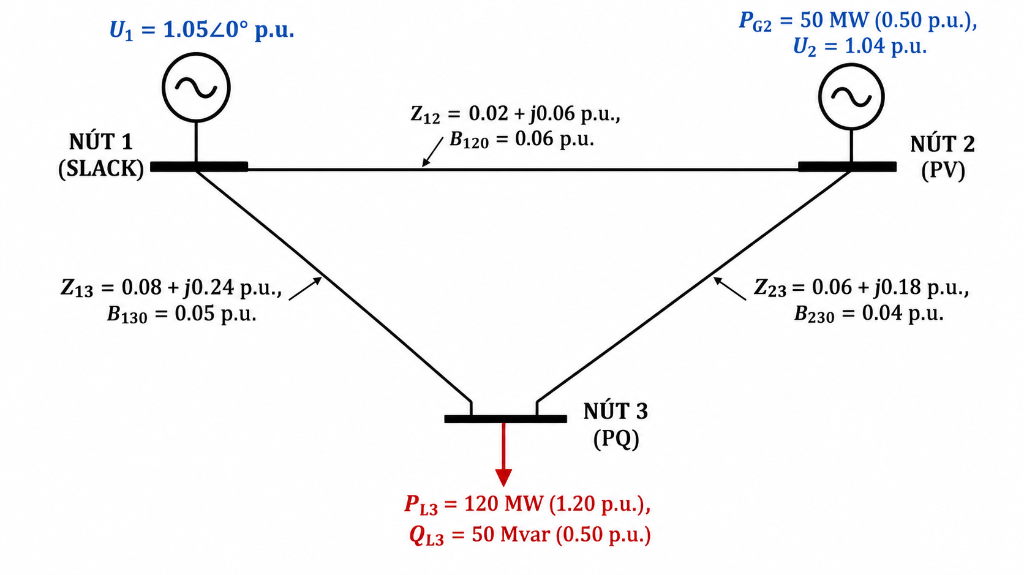
\includegraphics[width=0.65\textwidth]{../figures/3bus_network.png}
\caption{Single-line diagram of the benchmark 3-bus transmission network.}
\label{fig:3bus_sld}
\end{figure}

\section{Modeling Assumptions for Benchmark Verification and Scope Transition}
To establish a fully transparent, reproducible, and mathematically uncompromised numerical benchmark in Chapters 3 and 4, the following modeling assumptions are formally adopted:
\begin{enumerate}
    \item \textbf{Nominal Transformer Tap Ratios ($t = 1.0 + j0.0$):} All transmission branches are treated as direct bilateral transmission lines with nominal transformation ratios. This preserves full symmetry in the nodal admittance matrix ($Y_{ij} = Y_{ji}$).
    \item \textbf{Ideal Constant-Power Load Characteristic ($c_P = c_Q = 1.0; \; a_P = b_P = a_Q = b_Q = 0$):} Loads are modeled strictly as constant real and reactive power demands:
    \begin{equation}
    P_{Di}(U_i) = P_{Di0} = \text{const}, \qquad Q_{Di}(U_i) = Q_{Di0} = \text{const}
    \end{equation}
    This assumption serves as the standard industry benchmark for steady-state power flow verification. It represents the most demanding operating condition for numerical solvers because constant-power loads do not provide the natural voltage-relieving self-reduction characteristic inherent to constant-impedance loads ($\partial P_D / \partial U = 0$).
    \item \textbf{Jacobian Structure under Generalized Load Formulations:} If voltage-dependent ZIP loads are incorporated into the system model, the net scheduled injections become explicit functions of nodal voltage:
    \begin{equation}
    P_i^{\text{sch}}(U_i) = P_{Gi} - P_{Di}(U_i), \qquad Q_i^{\text{sch}}(U_i) = Q_{Gi} - Q_{Di}(U_i)
    \end{equation}
    Consequently, the power mismatch expressions become:
    \begin{equation}
    \Delta P_i(U) = P_{Gi} - P_{Di}(U_i) - P_i^{\text{calc}}(U, \delta), \qquad \Delta Q_i(U) = Q_{Gi} - Q_{Di}(U_i) - Q_i^{\text{calc}}(U, \delta)
    \end{equation}
    Differentiating these mismatches with respect to state variables reveals that the partial derivatives with respect to voltage magnitude acquire additional load derivative terms on the diagonal entries:
    \begin{equation}
    \frac{\partial (\Delta P_i)}{\partial U_i} = -\frac{\partial P_{Di}}{\partial U_i} - \frac{\partial P_i^{\text{calc}}}{\partial U_i}, \qquad \frac{\partial (\Delta Q_i)}{\partial U_i} = -\frac{\partial Q_{Di}}{\partial U_i} - \frac{\partial Q_i^{\text{calc}}}{\partial U_i}
    \end{equation}
    When formulating the linear Newton system $\mathbf{J} \Delta \mathbf{x} = \mathbf{f}$ where $\mathbf{J}$ represents the derivative of calculated power injections ($\mathbf{J} = \partial \mathbf{S}^{\text{calc}} / \partial \mathbf{x}$), the diagonal entries of blocks $\mathbf{N}$ ($J_{12}$) and $\mathbf{L}$ ($J_{22}$) must be explicitly augmented:
    \begin{equation}
    N_{ii}^{\text{ZIP}} = N_{ii} + \frac{\partial P_{Di}}{\partial U_i} = \left(\frac{P_i^{\text{calc}}}{U_i} + G_{ii} U_i\right) + P_{Di0} \left[ \frac{2 a_P U_i}{U_0^2} + \frac{b_P}{U_0} \right]
    \end{equation}
    \begin{equation}
    L_{ii}^{\text{ZIP}} = L_{ii} + \frac{\partial Q_{Di}}{\partial U_i} = \left(\frac{Q_i^{\text{calc}}}{U_i} - B_{ii} U_i\right) + Q_{Di0} \left[ \frac{2 a_Q U_i}{U_0^2} + \frac{b_Q}{U_0} \right]
    \end{equation}
    Under our adopted constant-power baseline ($a = b = 0, c = 1$), the voltage derivatives vanish identically ($\partial P_{Di}/\partial U_i = 0$ and $\partial Q_{Di}/\partial U_i = 0$), recovering the standard algebraic Jacobian formulation derived in Chapter 3.
\end{enumerate}

% ----------------------------------------------------
% CHAPTER 3: MATHEMATICAL FORMULATION & SOLVER
% ----------------------------------------------------
\chapter{Mathematical Formulation \& Newton--Raphson Solver}

\section{Non-Linear AC Nodal Power Flow Equations in Polar Coordinates}
Consider an $N$-bus power transmission network whose structural interconnection is represented by the complex nodal admittance matrix $\mathbf{Y}_{\text{bus}} \in \mathbb{C}^{N \times N}$, with elements $Y_{ij} = G_{ij} + jB_{ij}$. At any arbitrary bus $i$, the complex bus voltage phasor in polar coordinates is:
\begin{equation}
\dot{U}_i = U_i e^{j\delta_i} = U_i (\cos\delta_i + j\sin\delta_i)
\end{equation}
where $U_i = \vert{}\dot{U}_i\vert{}$ represents the voltage magnitude in per-unit, and $\delta_i$ denotes the voltage phase angle in radians.

From Kirchhoff's Current Law, the net complex current injected into the network at Bus $i$ is:
\begin{equation}
\dot{I}_i = \sum_{j=1}^N Y_{ij} \dot{U}_j = \sum_{j=1}^N (G_{ij} + jB_{ij}) U_j e^{j\delta_j}
\end{equation}
The complex apparent power injection at Bus $i$ is defined by complex power conservation:
\begin{equation}
S_i = P_i + jQ_i = \dot{U}_i \dot{I}_i^* = \left( U_i e^{j\delta_i} \right) \left[ \sum_{j=1}^N Y_{ij} U_j e^{j\delta_j} \right]^* = U_i e^{j\delta_i} \sum_{j=1}^N Y_{ij}^* U_j e^{-j\delta_j}
\end{equation}
Expanding this summation:
\begin{equation}
S_i = \sum_{j=1}^N U_i U_j Y_{ij}^* e^{j(\delta_i - \delta_j)}
\end{equation}

\subsection{Rectangular Admittance Representation ($G_{ij} + jB_{ij}$)}
Substituting the rectangular form $Y_{ij}^* = G_{ij} - jB_{ij}$ and applying Euler's identity $e^{j(\delta_i - \delta_j)} = \cos(\delta_i - \delta_j) + j\sin(\delta_i - \delta_j)$ with $\delta_{ij} = \delta_i - \delta_j$:
\begin{align}
S_i &= \sum_{j=1}^N U_i U_j (G_{ij} - jB_{ij}) [\cos\delta_{ij} + j\sin\delta_{ij}] \\
&= \sum_{j=1}^N U_i U_j \left[ (G_{ij}\cos\delta_{ij} + B_{ij}\sin\delta_{ij}) + j (G_{ij}\sin\delta_{ij} - B_{ij}\cos\delta_{ij}) \right]
\end{align}
Equating real and imaginary parts yields the standard non-linear AC power flow equations:
\begin{equation}
\label{eq:p_calc_rect}
P_i^{\text{calc}} = \sum_{j=1}^N U_i U_j (G_{ij} \cos\delta_{ij} + B_{ij} \sin\delta_{ij})
\end{equation}
\begin{equation}
\label{eq:q_calc_rect}
Q_i^{\text{calc}} = \sum_{j=1}^N U_i U_j (G_{ij} \sin\delta_{ij} - B_{ij} \cos\delta_{ij})
\end{equation}
where $\delta_{ij} = \delta_i - \delta_j$. Equations~\eqref{eq:p_calc_rect} and~\eqref{eq:q_calc_rect} represent the exact mathematical formulation implemented in our developed numerical solver.

\subsection{Polar Admittance Representation ($\vert{}Y_{ij}\vert{}\angle\theta_{ij}$)}
Alternatively, expressing admittance elements in polar form $Y_{ij} = \vert{}Y_{ij}\vert{} e^{j\theta_{ij}}$:
\begin{equation}
S_i = \sum_{j=1}^N U_i U_j \vert{}Y_{ij}\vert{} e^{-j\theta_{ij}} e^{j(\delta_i - \delta_j)} = \sum_{j=1}^N U_i U_j \vert{}Y_{ij}\vert{} e^{j(\delta_i - \delta_j - \theta_{ij})}
\end{equation}
Decomposing into real and imaginary parts:
\begin{equation}
P_i^{\text{calc}} = \sum_{j=1}^N U_i U_j \vert{}Y_{ij}\vert{} \cos(\delta_i - \delta_j - \theta_{ij})
\end{equation}
\begin{equation}
Q_i^{\text{calc}} = \sum_{j=1}^N U_i U_j \vert{}Y_{ij}\vert{} \sin(\delta_i - \delta_j - \theta_{ij})
\end{equation}

\section{Mismatch Vectors and Multivariable Taylor Series Linearization}
At each bus $i$, scheduled power injections are established from generation schedules and consumer load demands:
\begin{equation}
P_i^{\text{sch}} = P_{Gi} - P_{Di}, \qquad Q_i^{\text{sch}} = Q_{Gi} - Q_{Di}
\end{equation}
The power mismatches between scheduled net injections and non-linear calculated injections at iteration $m$ are defined as:
\begin{equation}
\Delta P_i^{(m)} = P_i^{\text{sch}} - P_i^{\text{calc}}( \boldsymbol{\delta}^{(m)}, \mathbf{U}^{(m)} )
\end{equation}
\begin{equation}
\Delta Q_i^{(m)} = Q_i^{\text{sch}} - Q_i^{\text{calc}}( \boldsymbol{\delta}^{(m)}, \mathbf{U}^{(m)} )
\end{equation}

The power flow problem seeks a state vector $\mathbf{x}^* = [\boldsymbol{\delta}^*, \mathbf{U}^*]^T$ such that all mismatches vanish simultaneously:
\begin{equation}
\mathbf{f}(\mathbf{x}^*) = \begin{bmatrix} \Delta \mathbf{P}(\boldsymbol{\delta}^*, \mathbf{U}^*) \\ \Delta \mathbf{Q}(\boldsymbol{\delta}^*, \mathbf{U}^*) \end{bmatrix} = \mathbf{0}
\end{equation}

Expanding the non-linear calculated power functions in a multivariable Taylor series around the current operating state $\mathbf{x}^{(m)} = [\boldsymbol{\delta}^{(m)}, \mathbf{U}^{(m)}]^T$:
\begin{equation}
P_i^{\text{calc}}(\mathbf{x}^{(m)} + \Delta \mathbf{x}) = P_i^{\text{calc}}(\mathbf{x}^{(m)}) + \sum_{j} \frac{\partial P_i}{\partial \delta_j} \Delta \delta_j + \sum_{j} \frac{\partial P_i}{\partial U_j} \Delta U_j + \mathcal{O}(\Vert\Delta \mathbf{x}\Vert^2)
\end{equation}
\begin{equation}
Q_i^{\text{calc}}(\mathbf{x}^{(m)} + \Delta \mathbf{x}) = Q_i^{\text{calc}}(\mathbf{x}^{(m)}) + \sum_{j} \frac{\partial Q_i}{\partial \delta_j} \Delta \delta_j + \sum_{j} \frac{\partial Q_i}{\partial U_j} \Delta U_j + \mathcal{O}(\Vert\Delta \mathbf{x}\Vert^2)
\end{equation}
Neglecting second- and higher-order terms ($\mathcal{O}(\Vert\Delta \mathbf{x}\Vert^2) \approx \mathbf{0}$) and setting the updated calculated power equal to scheduled injections yields the linearized system:
\begin{equation}
\begin{bmatrix} \Delta \mathbf{P}^{(m)} \\ \Delta \mathbf{Q}^{(m)} \end{bmatrix} = \begin{bmatrix} \mathbf{J}_{11}^{(m)} & \mathbf{J}_{12}^{(m)} \\ \mathbf{J}_{21}^{(m)} & \mathbf{J}_{22}^{(m)} \end{bmatrix} \begin{bmatrix} \Delta \boldsymbol{\delta}^{(m)} \\ \Delta \mathbf{U}^{(m)} \end{bmatrix}
\end{equation}
where the four Jacobian sub-matrices are conventionally denoted as:
\begin{equation}
\mathbf{J} = \begin{bmatrix} \mathbf{H} & \mathbf{N} \\ \mathbf{M} & \mathbf{L} \end{bmatrix} = \begin{bmatrix} \dfrac{\partial \mathbf{P}}{\partial \boldsymbol{\delta}} & \dfrac{\partial \mathbf{P}}{\partial \mathbf{U}} \\[8pt] \dfrac{\partial \mathbf{Q}}{\partial \boldsymbol{\delta}} & \dfrac{\partial \mathbf{Q}}{\partial \mathbf{U}} \end{bmatrix}
\end{equation}

\section{Analytical Closed-Form Derivation of the Four-Block Jacobian Sub-Matrices}
To avoid truncation and numerical inaccuracies associated with finite-difference approximations, our developed numerical solver computes all elements of the Jacobian matrix using exact analytical closed-form partial derivatives. For an $N$-bus power system, the complete derivations for all eight cases (diagonal $i=j$ and off-diagonal $i \neq j$ across all four blocks) are formulated as follows:

\subsection{Sub-Matrix Block H ($\mathbf{J}_{11} = \partial \mathbf{P} / \partial \boldsymbol{\delta}$)}
Expanding the calculated active power at Bus $i$ by isolating the diagonal $j = i$ term:
\begin{equation}
P_i = U_i^2 G_{ii} + \sum_{j \neq i} U_i U_j (G_{ij} \cos\delta_{ij} + B_{ij} \sin\delta_{ij})
\end{equation}

\subsubsection{Case 1: Off-Diagonal Elements ($i \neq j$)}
Differentiating with respect to $\delta_j$ (noting that $\partial \delta_{ij} / \partial \delta_j = \partial(\delta_i - \delta_j)/\partial \delta_j = -1$):
\begin{align}
H_{ij} = \frac{\partial P_i}{\partial \delta_j} &= U_i U_j \left[ -G_{ij} \sin\delta_{ij} \cdot (-1) + B_{ij} \cos\delta_{ij} \cdot (-1) \right] \nonumber \\
&= U_i U_j (G_{ij} \sin\delta_{ij} - B_{ij} \cos\delta_{ij}) \quad (i \neq j)
\end{align}

\subsubsection{Case 2: Diagonal Elements ($i = j$)}
Differentiating with respect to $\delta_i$ (noting that $\partial \delta_{ij} / \partial \delta_i = +1$):
\begin{equation}
H_{ii} = \frac{\partial P_i}{\partial \delta_i} = \sum_{j \neq i} U_i U_j (-G_{ij} \sin\delta_{ij} + B_{ij} \cos\delta_{ij})
\end{equation}
Recall the reactive power injection equation from Eq.~\eqref{eq:q_calc_rect}:
\begin{equation}
Q_i = -U_i^2 B_{ii} + \sum_{j \neq i} U_i U_j (G_{ij} \sin\delta_{ij} - B_{ij} \cos\delta_{ij})
\end{equation}
Rearranging this summation yields:
\begin{equation}
\sum_{j \neq i} U_i U_j (G_{ij} \sin\delta_{ij} - B_{ij} \cos\delta_{ij}) = Q_i + U_i^2 B_{ii}
\end{equation}
Negating both sides and substituting into the diagonal expression:
\begin{equation}
H_{ii} = \frac{\partial P_i}{\partial \delta_i} = -Q_i - B_{ii} U_i^2
\end{equation}

\subsection{Sub-Matrix Block N ($\mathbf{J}_{12} = \partial \mathbf{P} / \partial \mathbf{U}$)}

\subsubsection{Case 3: Off-Diagonal Elements ($i \neq j$)}
Differentiating $P_i$ with respect to voltage magnitude $U_j$:
\begin{equation}
N_{ij} = \frac{\partial P_i}{\partial U_j} = U_i (G_{ij} \cos\delta_{ij} + B_{ij} \sin\delta_{ij}) \quad (i \neq j)
\end{equation}

\subsubsection{Case 4: Diagonal Elements ($i = j$)}
Differentiating $P_i$ with respect to its own voltage magnitude $U_i$:
\begin{equation}
N_{ii} = \frac{\partial P_i}{\partial U_i} = 2 U_i G_{ii} + \sum_{j \neq i} U_j (G_{ij} \cos\delta_{ij} + B_{ij} \sin\delta_{ij})
\end{equation}
From the active power equation, the summation term can be expressed in terms of $P_i$:
\begin{equation}
\sum_{j \neq i} U_j (G_{ij} \cos\delta_{ij} + B_{ij} \sin\delta_{ij}) = \frac{P_i - U_i^2 G_{ii}}{U_i} = \frac{P_i}{U_i} - U_i G_{ii}
\end{equation}
Substituting this relation into the diagonal expression:
\begin{equation}
N_{ii} = \frac{\partial P_i}{\partial U_i} = 2 U_i G_{ii} + \left( \frac{P_i}{U_i} - U_i G_{ii} \right) = \frac{P_i}{U_i} + G_{ii} U_i
\end{equation}

\subsection{Sub-Matrix Block M ($\mathbf{J}_{21} = \partial \mathbf{Q} / \partial \boldsymbol{\delta}$)}
Expanding the calculated reactive power at Bus $i$:
\begin{equation}
Q_i = -U_i^2 B_{ii} + \sum_{j \neq i} U_i U_j (G_{ij} \sin\delta_{ij} - B_{ij} \cos\delta_{ij})
\end{equation}

\subsubsection{Case 5: Off-Diagonal Elements ($i \neq j$)}
Differentiating with respect to $\delta_j$ (with $\partial \delta_{ij} / \partial \delta_j = -1$):
\begin{align}
M_{ij} = \frac{\partial Q_i}{\partial \delta_j} &= U_i U_j \left[ G_{ij} \cos\delta_{ij} \cdot (-1) - B_{ij} (-\sin\delta_{ij}) \cdot (-1) \right] \nonumber \\
&= -U_i U_j (G_{ij} \cos\delta_{ij} + B_{ij} \sin\delta_{ij}) \quad (i \neq j)
\end{align}

\subsubsection{Case 6: Diagonal Elements ($i = j$)}
Differentiating with respect to $\delta_i$ (with $\partial \delta_{ij} / \partial \delta_i = +1$):
\begin{equation}
M_{ii} = \frac{\partial Q_i}{\partial \delta_i} = \sum_{j \neq i} U_i U_j (G_{ij} \cos\delta_{ij} + B_{ij} \sin\delta_{ij})
\end{equation}
From the active power expression $P_i = U_i^2 G_{ii} + \sum_{j \neq i} U_i U_j (G_{ij} \cos\delta_{ij} + B_{ij} \sin\delta_{ij})$, we directly obtain:
\begin{equation}
M_{ii} = \frac{\partial Q_i}{\partial \delta_i} = P_i - G_{ii} U_i^2
\end{equation}

\subsection{Sub-Matrix Block L ($\mathbf{J}_{22} = \partial \mathbf{Q} / \partial \mathbf{U}$)}

\subsubsection{Case 7: Off-Diagonal Elements ($i \neq j$)}
Differentiating $Q_i$ with respect to voltage magnitude $U_j$:
\begin{equation}
L_{ij} = \frac{\partial Q_i}{\partial U_j} = U_i (G_{ij} \sin\delta_{ij} - B_{ij} \cos\delta_{ij}) \quad (i \neq j)
\end{equation}

\subsubsection{Case 8: Diagonal Elements ($i = j$)}
Differentiating $Q_i$ with respect to its own voltage magnitude $U_i$:
\begin{equation}
L_{ii} = \frac{\partial Q_i}{\partial U_i} = -2 U_i B_{ii} + \sum_{j \neq i} U_j (G_{ij} \sin\delta_{ij} - B_{ij} \cos\delta_{ij})
\end{equation}
From the reactive power expression:
\begin{equation}
\sum_{j \neq i} U_j (G_{ij} \sin\delta_{ij} - B_{ij} \cos\delta_{ij}) = \frac{Q_i + U_i^2 B_{ii}}{U_i} = \frac{Q_i}{U_i} + U_i B_{ii}
\end{equation}
Substituting this relation into the diagonal expression:
\begin{equation}
L_{ii} = \frac{\partial Q_i}{\partial U_i} = -2 U_i B_{ii} + \left( \frac{Q_i}{U_i} + U_i B_{ii} \right) = \frac{Q_i}{U_i} - B_{ii} U_i
\end{equation}

\subsection{Summary of Closed-Form Jacobian Formulas}
Table~\ref{tab:jacobian_formulas} summarizes the closed-form analytical formulas implemented in our developed numerical solver.

\begin{table}[H]
\centering
\caption{Closed-form analytical partial derivative formulas of the polar Jacobian matrix.}
\label{tab:jacobian_formulas}
\begin{tabular}{lll}
\toprule
\textbf{Block} & \textbf{Off-Diagonal ($i \neq j$)} & \textbf{Diagonal ($i = j$)} \\
\midrule
$\mathbf{H} = \dfrac{\partial \mathbf{P}}{\partial \boldsymbol{\delta}}$ & $H_{ij} = U_i U_j (G_{ij}\sin\delta_{ij} - B_{ij}\cos\delta_{ij})$ & $H_{ii} = -Q_i - B_{ii} U_i^2$ \\[8pt]
$\mathbf{N} = \dfrac{\partial \mathbf{P}}{\partial \mathbf{U}}$ & $N_{ij} = U_i (G_{ij}\cos\delta_{ij} + B_{ij}\sin\delta_{ij})$ & $N_{ii} = \dfrac{P_i}{U_i} + G_{ii} U_i$ \\[8pt]
$\mathbf{M} = \dfrac{\partial \mathbf{Q}}{\partial \boldsymbol{\delta}}$ & $M_{ij} = -U_i U_j (G_{ij}\cos\delta_{ij} + B_{ij}\sin\delta_{ij})$ & $M_{ii} = P_i - G_{ii} U_i^2$ \\[8pt]
$\mathbf{L} = \dfrac{\partial \mathbf{Q}}{\partial \mathbf{U}}$ & $L_{ij} = U_i (G_{ij}\sin\delta_{ij} - B_{ij}\cos\delta_{ij})$ & $L_{ii} = \dfrac{Q_i}{U_i} - B_{ii} U_i$ \\
\bottomrule
\end{tabular}
\end{table}

\section{Iterative Solution Algorithm, Stopping Criteria, and Q-Limit Handling}

\subsection{State Vector Updating and Unit Discipline}
At each iteration $m$, the linear matrix equation is solved:
\begin{equation}
\mathbf{J}^{(m)} \Delta \mathbf{x}^{(m)} = \begin{bmatrix} \Delta \mathbf{P}^{(m)} \\ \Delta \mathbf{Q}^{(m)} \end{bmatrix}
\end{equation}
where the state correction vector is partitioned as:
\begin{equation}
\Delta \mathbf{x}^{(m)} = \begin{bmatrix} \Delta \boldsymbol{\delta}^{(m)} \\ \Delta \mathbf{U}^{(m)} \end{bmatrix}
\end{equation}
\begin{itemize}
    \item $\Delta \boldsymbol{\delta}^{(m)} \in \mathbb{R}^{N-1}$: Phase angle corrections for all non-slack buses, solved in \textbf{radians (rad)}.
    \item $\Delta \mathbf{U}^{(m)} \in \mathbb{R}^{N_{\text{PQ}}}$: Voltage magnitude corrections for all PQ load buses, solved in \textbf{per-unit (p.u.)}.
\end{itemize}

The updated state variables for iteration $m+1$ are computed via:
\begin{equation}
\delta_i^{(m+1)} = \delta_i^{(m)} + \Delta \delta_i^{(m)} \quad (i \in \text{non-slack buses})
\end{equation}
\begin{equation}
U_i^{(m+1)} = U_i^{(m)} + \Delta U_i^{(m)} \quad (i \in \text{PQ buses})
\end{equation}
\textbf{Unit Discipline:} When updating angle tables or presenting results to engineers, phase angle corrections in radians are converted to degrees via:
\begin{equation}
\Delta \delta_i^\circ = \Delta \delta_i^{\text{rad}} \times \frac{180^\circ}{\pi}
\end{equation}

\subsection{Stopping Criteria}
The iteration continues until the maximum absolute power mismatch across all active and reactive power balance equations satisfies the infinite-norm convergence threshold:
\begin{equation}
\Vert \mathbf{f}^{(m)} \Vert_\infty = \max \left( \max_{i \in \text{non-slack}} \vert{}\Delta P_i^{(m)}\vert{}, \; \max_{i \in \text{PQ}} \vert{}\Delta Q_i^{(m)}\vert{} \right) \le \varepsilon = 10^{-10}\text{ p.u.}
\end{equation}
If the iteration count exceeds $m_{\max} = 30$ without satisfying this criterion, the algorithm terminates with an unconverged status, signaling potential voltage collapse or ill-conditioned system data.

\section{Post-Convergence Network Calculations}
Once the state vector $[\boldsymbol{\delta}^*, \mathbf{U}^*]^T$ converges, secondary physical network variables are evaluated:

\subsection{Slack and PV Bus Generations}
The active and reactive power generated at the Slack bus (Bus 1) are calculated from the network injections:
\begin{equation}
P_{G1} = P_1^{\text{calc}} + P_{D1}, \qquad Q_{G1} = Q_1^{\text{calc}} + Q_{D1}
\end{equation}
For each PV generator bus $k$, the reactive power duty is:
\begin{equation}
Q_{Gk} = Q_k^{\text{calc}} + Q_{Dk}
\end{equation}

\subsection{Complex Branch Power Flows}
For each branch connecting Bus $i$ and Bus $j$, the complex current phasor flowing from Bus $i$ toward Bus $j$ is:
\begin{equation}
\dot{I}_{ij} = \frac{\dot{U}_i - \dot{U}_j}{z_{ij}} + j \frac{B_{ij}}{2} \dot{U}_i
\end{equation}
The complex power flow leaving Bus $i$ toward Bus $j$ is:
\begin{equation}
S_{ij} = P_{ij} + jQ_{ij} = \dot{U}_i \dot{I}_{ij}^* = U_i e^{j\delta_i} \left[ \frac{U_i e^{-j\delta_i} - U_j e^{-j\delta_j}}{r_{ij} - jx_{ij}} - j \frac{B_{ij}}{2} U_i e^{-j\delta_i} \right]
\end{equation}
Similarly, the complex power flow arriving at Bus $j$ from Bus $i$ is:
\begin{equation}
S_{ji} = P_{ji} + jQ_{ji} = \dot{U}_j \dot{I}_{ji}^* = U_j e^{j\delta_j} \left[ \frac{U_j e^{-j\delta_j} - U_i e^{-j\delta_i}}{r_{ij} - jx_{ij}} - j \frac{B_{ij}}{2} U_j e^{-j\delta_j} \right]
\end{equation}

\subsection{Transmission Losses and Global Energy Balance Audit}
The complex transmission power loss along branch $i-j$ is the sum of terminal power flows:
\begin{equation}
\Delta S_{ij} = S_{ij} + S_{ji} = \Delta P_{ij} + j\Delta Q_{ij}
\end{equation}
The active power dissipation ($\Delta P_{ij}$) represents Joule heating:
\begin{equation}
\Delta P_{ij} = \vert{}\dot{I}_{\text{series}, ij}\vert{}^2 r_{ij} = \left\vert{} \frac{\dot{U}_i - \dot{U}_j}{z_{ij}} \right\vert{}^2 r_{ij}
\end{equation}
The total system active and reactive losses are:
\begin{equation}
\Delta P_{\Sigma} = \sum_{\text{all branches}} \Delta P_{ij}, \qquad \Delta Q_{\Sigma} = \sum_{\text{all branches}} \Delta Q_{ij}
\end{equation}

Global network conservation of energy requires that total generation balances total demand plus losses:
\begin{equation}
\label{eq:p_balance}
\sum_{i=1}^N P_{Gi} - \sum_{i=1}^N P_{Di} - \Delta P_{\Sigma} = 0.000000\text{ MW}
\end{equation}
\begin{equation}
\label{eq:q_balance}
\sum_{i=1}^N Q_{Gi} - \sum_{i=1}^N Q_{Di} - \Delta Q_{\Sigma} = 0.000000\text{ Mvar}
\end{equation}

\section{Complete Algorithm Flowchart}
Figure~\ref{fig:algorithm_flowchart} illustrates the computational flowchart of the Newton--Raphson solver.

\begin{figure}[H]
\centering
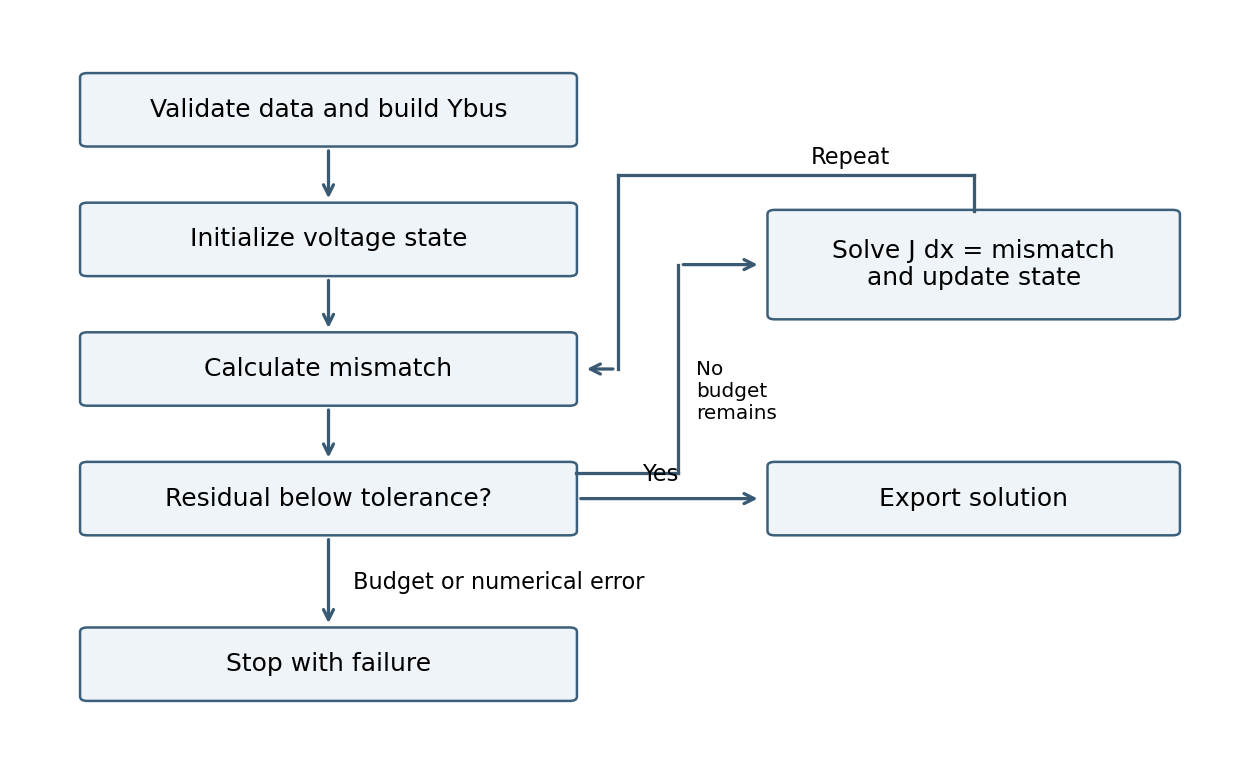
\includegraphics[width=0.75\textwidth]{../figures/algorithm.png}
\caption{Flowchart of the polar Newton--Raphson power flow solver.}
\label{fig:algorithm_flowchart}
\end{figure}

% ----------------------------------------------------
% CHAPTER 4: NUMERICAL VERIFICATION & TEST SCENARIOS
% ----------------------------------------------------
\chapter{Numerical Verification \& Operational Scenario Analysis}

\section{Detailed Step-by-Step Hand Calculation on the 3-Bus Benchmark Network (Iteration $m = 0 \to 1$)}

\subsection{Network Topology and Specified Input Parameters}
The test transmission system consists of 3 buses: Bus 1 (Slack), Bus 2 (PV generator), and Bus 3 (PQ load), operating on a three-phase system base of $S_{\text{base}} = 100.0\text{ MVA}$ at $f = 50\text{ Hz}$.

\begin{table}[H]
\centering
\caption{Nodal input data for the benchmark 3-bus transmission network.}
\label{tab:3bus_bus_data}
\begin{tabular}{ccccccccc}
\toprule
\textbf{Bus} & \textbf{Type} & \textbf{$U_{\text{spec}}$ (p.u.)} & \textbf{$\delta_{\text{spec}}$ (deg)} & \textbf{$P_G$ (p.u.)} & \textbf{$Q_G$ (p.u.)} & \textbf{$P_D$ (p.u.)} & \textbf{$Q_D$ (p.u.)} & \textbf{$P^{\text{sch}}$ / $Q^{\text{sch}}$} \\
\midrule
1 & Slack & 1.050000 & 0.000000 & Unspec. & Unspec. & 0.000000 & 0.000000 & --- \\
2 & PV & 1.020000 & 0.000000 & 0.500000 & Unspec. & 0.000000 & 0.000000 & $P_2^{\text{sch}} = +0.500000$ \\
3 & PQ & 1.000000 & 0.000000 & 0.000000 & 0.000000 & 0.600000 & 0.250000 & $P_3^{\text{sch}} = -0.600000$ \\
  &    &          &          &          &          &          &          & $Q_3^{\text{sch}} = -0.250000$ \\
\bottomrule
\end{tabular}
\end{table}

\begin{table}[H]
\centering
\caption{Branch transmission line parameters on $100.0\text{ MVA}$ base.}
\label{tab:3bus_line_data}
\begin{tabular}{ccccc}
\toprule
\textbf{Branch} & \textbf{From Bus} & \textbf{To Bus} & \textbf{Series Resistance $r_{ij}$ (p.u.)} & \textbf{Series Reactance $x_{ij}$ (p.u.)} \\
\midrule
1 & 1 & 2 & 0.020000 & 0.060000 \\
2 & 1 & 3 & 0.080000 & 0.240000 \\
3 & 2 & 3 & 0.060000 & 0.180000 \\
\bottomrule
\end{tabular}
\end{table}

\subsection{Explicit Construction of Primitive Admittances and $Y_{\text{bus}}$}
Calculating primitive series admittances $y_{ij} = z_{ij}^{-1} = \frac{r_{ij} - jx_{ij}}{r_{ij}^2 + x_{ij}^2}$:
\begin{equation}
y_{12} = \frac{1}{0.02 + j0.06} = \frac{0.02 - j0.06}{0.02^2 + 0.06^2} = \frac{0.02 - j0.06}{0.0040} = 5.000000 - j15.000000\text{ p.u.}
\end{equation}
\begin{equation}
y_{13} = \frac{1}{0.08 + j0.24} = \frac{0.08 - j0.24}{0.08^2 + 0.24^2} = \frac{0.08 - j0.24}{0.0640} = 1.250000 - j3.750000\text{ p.u.}
\end{equation}
\begin{equation}
y_{23} = \frac{1}{0.06 + j0.18} = \frac{0.06 - j0.18}{0.06^2 + 0.18^2} = \frac{0.06 - j0.18}{0.0360} = 1.666667 - j5.000000\text{ p.u.}
\end{equation}

Constructing diagonal and off-diagonal elements of $\mathbf{Y}_{\text{bus}}$ ($b_{ij0} = 0$):
\begin{equation}
Y_{11} = y_{12} + y_{13} = (5.0 - j15.0) + (1.25 - j3.75) = 6.250000 - j18.750000\text{ p.u.}
\end{equation}
\begin{equation}
Y_{12} = Y_{21} = -y_{12} = -5.000000 + j15.000000\text{ p.u.}
\end{equation}
\begin{equation}
Y_{13} = Y_{31} = -y_{13} = -1.250000 + j3.750000\text{ p.u.}
\end{equation}
\begin{equation}
Y_{22} = y_{12} + y_{23} = (5.0 - j15.0) + (1.666667 - j5.0) = 6.666667 - j20.000000\text{ p.u.}
\end{equation}
\begin{equation}
Y_{23} = Y_{32} = -y_{23} = -1.666667 + j5.000000\text{ p.u.}
\end{equation}
\begin{equation}
Y_{33} = y_{13} + y_{23} = (1.25 - j3.75) + (1.666667 - j5.0) = 2.916667 - j8.750000\text{ p.u.}
\end{equation}

In matrix format:
\begin{equation}
\mathbf{Y}_{\text{bus}} = \begin{bmatrix}
6.250000 - j18.750000 & -5.000000 + j15.000000 & -1.250000 + j3.750000 \\
-5.000000 + j15.000000 & 6.666667 - j20.000000 & -1.666667 + j5.000000 \\
-1.250000 + j3.750000 & -1.666667 + j5.000000 & 2.916667 - j8.750000
\end{bmatrix}\text{ p.u.}
\end{equation}

\subsection{Flat-Start Initialization ($m = 0$) and Initial Power Injections and Mismatches}
The initial state vector at iteration $m = 0$ is initialized via standard flat start:
\begin{equation}
U_1^{(0)} = 1.050000\text{ p.u.}, \quad U_2^{(0)} = 1.020000\text{ p.u.}, \quad U_3^{(0)} = 1.000000\text{ p.u.}
\end{equation}
\begin{equation}
\delta_1^{(0)} = 0.000000\text{ rad}, \quad \delta_2^{(0)} = 0.000000\text{ rad}, \quad \delta_3^{(0)} = 0.000000\text{ rad}
\end{equation}
Since all phase angles are zero, $\delta_{ij}^{(0)} = 0$, leading to $\cos\delta_{ij}^{(0)} = 1$ and $\sin\delta_{ij}^{(0)} = 0$.

\subsubsection{Calculated Active Power Injections at $m = 0$:}
\begin{align}
P_2^{\text{calc},(0)} &= U_2^{(0)} \left[ U_1^{(0)} G_{21} + U_2^{(0)} G_{22} + U_3^{(0)} G_{23} \right] \nonumber \\
&= 1.02 \left[ 1.05(-5.0) + 1.02(6.666667) + 1.0(-1.666667) \right] \nonumber \\
&= 1.02 \left[ -5.250000 + 6.800000 - 1.666667 \right] = 1.02 \left[ -0.116667 \right] = -0.119000\text{ p.u.}
\end{align}
\begin{align}
P_3^{\text{calc},(0)} &= U_3^{(0)} \left[ U_1^{(0)} G_{31} + U_2^{(0)} G_{32} + U_3^{(0)} G_{33} \right] \nonumber \\
&= 1.00 \left[ 1.05(-1.25) + 1.02(-1.666667) + 1.0(2.916667) \right] \nonumber \\
&= 1.00 \left[ -1.312500 - 1.700000 + 2.916667 \right] = -0.095833\text{ p.u.}
\end{align}

\subsubsection{Calculated Reactive Power Injection at $m = 0$:}
\begin{align}
Q_3^{\text{calc},(0)} &= U_3^{(0)} \left[ -U_1^{(0)} B_{31} - U_2^{(0)} B_{32} - U_3^{(0)} B_{33} \right] \nonumber \\
&= 1.00 \left[ -1.05(3.75) - 1.02(5.0) - 1.0(-8.75) \right] \nonumber \\
&= 1.00 \left[ -3.937500 - 5.100000 + 8.750000 \right] = -0.287500\text{ p.u.}
\end{align}

\subsubsection{Power Mismatches at $m = 0$:}
\begin{equation}
\Delta P_2^{(0)} = P_2^{\text{sch}} - P_2^{\text{calc},(0)} = 0.500000 - (-0.119000) = +0.619000\text{ p.u.}
\end{equation}
\begin{equation}
\Delta P_3^{(0)} = P_3^{\text{sch}} - P_3^{\text{calc},(0)} = -0.600000 - (-0.095833) = -0.504167\text{ p.u.}
\end{equation}
\begin{equation}
\Delta Q_3^{(0)} = Q_3^{\text{sch}} - Q_3^{\text{calc},(0)} = -0.250000 - (-0.287500) = +0.037500\text{ p.u.}
\end{equation}
\begin{equation}
\mathbf{f}^{(0)} = \begin{bmatrix} \Delta P_2^{(0)} \\ \Delta P_3^{(0)} \\ \Delta Q_3^{(0)} \end{bmatrix} = \begin{bmatrix} +0.619000 \\ -0.504167 \\ +0.037500 \end{bmatrix}
\end{equation}

\subsection{Analytical Element-by-Element Evaluation of the Initial Jacobian Matrix $J^{(0)}$}
The state correction vector is $\Delta \mathbf{x}^{(0)} = [\Delta \delta_2^{(0)}, \Delta \delta_3^{(0)}, \Delta U_3^{(0)}]^T$. The Jacobian $\mathbf{J}^{(0)} \in \mathbb{R}^{3 \times 3}$ is evaluated element-by-element:

\subsubsection{Row 1 ($\Delta P_2$ Derivatives):}
\begin{itemize}
    \item $J_{11}^{(0)} = H_{22}^{(0)} = -Q_2^{\text{calc},(0)} - B_{22} (U_2^{(0)})^2$.
    First evaluate $Q_2^{\text{calc},(0)}$:
    \begin{align}
    Q_2^{\text{calc},(0)} &= U_2^{(0)} \left[ -U_1^{(0)} B_{21} - U_2^{(0)} B_{22} - U_3^{(0)} B_{23} \right] \nonumber \\
    &= 1.02 \left[ -1.05(15.0) - 1.02(-20.0) - 1.0(5.0) \right] \nonumber \\
    &= 1.02 \left[ -15.750000 + 20.400000 - 5.000000 \right] = 1.02(-0.35) = -0.357000\text{ p.u.}
    \end{align}
    Then:
    \begin{equation}
    H_{22}^{(0)} = -(-0.357000) - (-20.0)(1.02)^2 = 0.357000 + 20.0(1.0404) = 21.165000
    \end{equation}
    \item $J_{12}^{(0)} = H_{23}^{(0)} = U_2^{(0)} U_3^{(0)} (G_{23} \sin 0 - B_{23} \cos 0) = -U_2^{(0)} U_3^{(0)} B_{23} = -(1.02)(1.0)(5.0) = -5.100000$
    \item $J_{13}^{(0)} = N_{23}^{(0)} = U_2^{(0)} (G_{23} \cos 0 + B_{23} \sin 0) = U_2^{(0)} G_{23} = (1.02)(-1.666667) = -1.700000$
\end{itemize}

\subsubsection{Row 2 ($\Delta P_3$ Derivatives):}
\begin{itemize}
    \item $J_{21}^{(0)} = H_{32}^{(0)} = -U_3^{(0)} U_2^{(0)} B_{32} = -(1.0)(1.02)(5.0) = -5.100000$
    \item $J_{22}^{(0)} = H_{33}^{(0)} = -Q_3^{\text{calc},(0)} - B_{33} (U_3^{(0)})^2 = -(-0.287500) - (-8.750000)(1.0)^2 = 0.287500 + 8.750000 = 9.037500$
    \item $J_{23}^{(0)} = N_{33}^{(0)} = \dfrac{P_3^{\text{calc},(0)}}{U_3^{(0)}} + G_{33} U_3^{(0)} = \dfrac{-0.095833}{1.0} + (2.916667)(1.0) = 2.820833$
\end{itemize}

\subsubsection{Row 3 ($\Delta Q_3$ Derivatives):}
\begin{itemize}
    \item $J_{31}^{(0)} = M_{32}^{(0)} = -U_3^{(0)} U_2^{(0)} G_{32} = -(1.0)(1.02)(-1.666667) = +1.700000$
    \item $J_{32}^{(0)} = M_{33}^{(0)} = P_3^{\text{calc},(0)} - G_{33} (U_3^{(0)})^2 = -0.095833 - (2.916667)(1.0)^2 = -3.012500$
    \item $J_{33}^{(0)} = L_{33}^{(0)} = \dfrac{Q_3^{\text{calc},(0)}}{U_3^{(0)}} - B_{33} U_3^{(0)} = \dfrac{-0.287500}{1.0} - (-8.750000)(1.0) = -0.287500 + 8.750000 = 8.462500$
\end{itemize}

Assembling the complete initial Jacobian matrix $\mathbf{J}^{(0)}$:
\begin{equation}
\mathbf{J}^{(0)} = \begin{bmatrix}
21.165000 & -5.100000 & -1.700000 \\
-5.100000 & 9.037500 & 2.820833 \\
1.700000 & -3.012500 & 8.462500
\end{bmatrix}
\end{equation}

\subsection{Linear System Inversion and First State Correction Vector Update ($x^{(1)}$)}
Setting up the system $\mathbf{J}^{(0)} \Delta \mathbf{x}^{(0)} = \mathbf{f}^{(0)}$:
\begin{equation}
\begin{bmatrix}
21.165000 & -5.100000 & -1.700000 \\
-5.100000 & 9.037500 & 2.820833 \\
1.700000 & -3.012500 & 8.462500
\end{bmatrix}
\begin{bmatrix}
\Delta \delta_2^{(0)} \\
\Delta \delta_3^{(0)} \\
\Delta U_3^{(0)}
\end{bmatrix}
=
\begin{bmatrix}
+0.619000 \\
-0.504167 \\
+0.037500
\end{bmatrix}
\end{equation}

Solving via Gaussian elimination yields the exact state correction vector:
\begin{equation}
\Delta \delta_2^{(0)} = +0.01820908\text{ rad} = +1.043303^\circ
\end{equation}
\begin{equation}
\Delta \delta_3^{(0)} = -0.04117662\text{ rad} = -2.359247^\circ
\end{equation}
\begin{equation}
\Delta U_3^{(0)} = -0.01388479\text{ p.u.}
\end{equation}

Updating the nodal state variables for Iteration 1 ($m = 1$):
\begin{equation}
\delta_2^{(1)} = \delta_2^{(0)} + \Delta \delta_2^{(0)} = 0.0 + 0.01820908 = +0.01820908\text{ rad} \quad (+1.043303^\circ)
\end{equation}
\begin{equation}
\delta_3^{(1)} = \delta_3^{(0)} + \Delta \delta_3^{(0)} = 0.0 - 0.04117662 = -0.04117662\text{ rad} \quad (-2.359247^\circ)
\end{equation}
\begin{equation}
U_3^{(1)} = U_3^{(0)} + \Delta U_3^{(0)} = 1.00000000 - 0.01388479 = 0.98611521\text{ p.u.}
\end{equation}

\section{Multi-Tier Software Cross-Validation}

\subsection{Iteration 1 Cross-Validation Table}
Table~\ref{tab:iter1_validation} compares each intermediate and updated quantity at $m = 1$ between the manual hand calculations and the developed numerical solver.

\begin{table}[H]
\centering
\caption{Iteration 1 numerical cross-validation (Hand Calculation vs. Developed Solver).}
\label{tab:iter1_validation}
\begin{tabular}{lcccc}
\toprule
\textbf{Variable} & \textbf{Hand Calculation} & \textbf{Developed Solver} & \textbf{Absolute Discrepancy} & \textbf{Status} \\
\midrule
$P_2^{\text{calc},(0)}$ (p.u.) & -0.119000 & -0.119000 & $0.000000$ & Exact \\
$P_3^{\text{calc},(0)}$ (p.u.) & -0.095833 & -0.095833 & $< 10^{-16}$ & Exact \\
$Q_3^{\text{calc},(0)}$ (p.u.) & -0.287500 & -0.287500 & $0.000000$ & Exact \\
$\Delta P_2^{(0)}$ (p.u.) & +0.619000 & +0.619000 & $0.000000$ & Exact \\
$\Delta P_3^{(0)}$ (p.u.) & -0.504167 & -0.504167 & $< 10^{-16}$ & Exact \\
$\Delta Q_3^{(0)}$ (p.u.) & +0.037500 & +0.037500 & $0.000000$ & Exact \\
$J_{11}^{(0)}$ ($H_{22}$) & 21.165000 & 21.165000 & $0.000000$ & Exact \\
$J_{12}^{(0)}$ ($H_{23}$) & -5.100000 & -5.100000 & $0.000000$ & Exact \\
$J_{13}^{(0)}$ ($N_{23}$) & -1.700000 & -1.700000 & $0.000000$ & Exact \\
$J_{21}^{(0)}$ ($H_{32}$) & -5.100000 & -5.100000 & $0.000000$ & Exact \\
$J_{22}^{(0)}$ ($H_{33}$) & 9.037500 & 9.037500 & $0.000000$ & Exact \\
$J_{23}^{(0)}$ ($N_{33}$) & 2.820833 & 2.820833 & $< 10^{-16}$ & Exact \\
$J_{31}^{(0)}$ ($M_{32}$) & 1.700000 & 1.700000 & $0.000000$ & Exact \\
$J_{32}^{(0)}$ ($M_{33}$) & -3.012500 & -3.012500 & $0.000000$ & Exact \\
$J_{33}^{(0)}$ ($L_{33}$) & 8.462500 & 8.462500 & $0.000000$ & Exact \\
$\Delta \delta_2^{(0)}$ (rad) & +0.01820908 & +0.01820908 & $< 10^{-16}$ & Exact \\
$\Delta \delta_3^{(0)}$ (rad) & -0.04117662 & -0.04117662 & $< 10^{-16}$ & Exact \\
$\Delta U_3^{(0)}$ (p.u.) & -0.01388479 & -0.01388479 & $< 10^{-16}$ & Exact \\
$\delta_2^{(1)}$ (deg) & +1.043303 & +1.043303 & $< 10^{-15}$ & Exact \\
$\delta_3^{(1)}$ (deg) & -2.359247 & -2.359247 & $< 10^{-15}$ & Exact \\
$U_3^{(1)}$ (p.u.) & 0.986115 & 0.986115 & $< 10^{-16}$ & Exact \\
\bottomrule
\end{tabular}
\end{table}

\subsection{Full Convergence Trajectory Audit}
Table~\ref{tab:convergence_audit} details the iteration-by-iteration convergence trajectory of the solver under a stopping threshold of $\varepsilon = 10^{-10}\text{ p.u.}$

\begin{table}[H]
\centering
\caption{Iteration-by-iteration convergence trajectory of the Newton--Raphson solver.}
\label{tab:convergence_audit}
\begin{tabular}{cccccc}
\toprule
\textbf{Iter ($m$)} & \textbf{$U_3^{(m)}$ (p.u.)} & \textbf{$\delta_2^{(m)}$ (deg)} & \textbf{$\delta_3^{(m)}$ (deg)} & \textbf{$\Vert \mathbf{f}^{(m)} \Vert_\infty$ (p.u.)} & \textbf{Convergence Status} \\
\midrule
0 & 1.000000 & 0.000000 & 0.000000 & $6.1900 \times 10^{-1}$ & Initial Flat Start \\
1 & 0.986115 & +1.043303 & -2.359247 & $1.1618 \times 10^{-2}$ & Active Iteration \\
2 & 0.984386 & +1.024102 & -2.418296 & $2.4284 \times 10^{-5}$ & Active Iteration \\
3 & 0.984385 & +1.024098 & -2.418330 & $1.0454 \times 10^{-10}$ & Active Iteration \\
4 & 0.984385 & +1.024098 & -2.418330 & $6.1062 \times 10^{-16}$ & \textbf{Converged ($\le 10^{-10}$)} \\
\bottomrule
\end{tabular}
\end{table}

The maximum mismatch drops from $6.19 \times 10^{-1}$ to $1.16 \times 10^{-2}$, then to $2.43 \times 10^{-5}$, and finally to $1.05 \times 10^{-10}$, demonstrating the quadratic convergence property ($\Vert \mathbf{f}^{(m+1)} \Vert \le C \Vert \mathbf{f}^{(m)} \Vert^2$).

\begin{figure}[H]
\centering
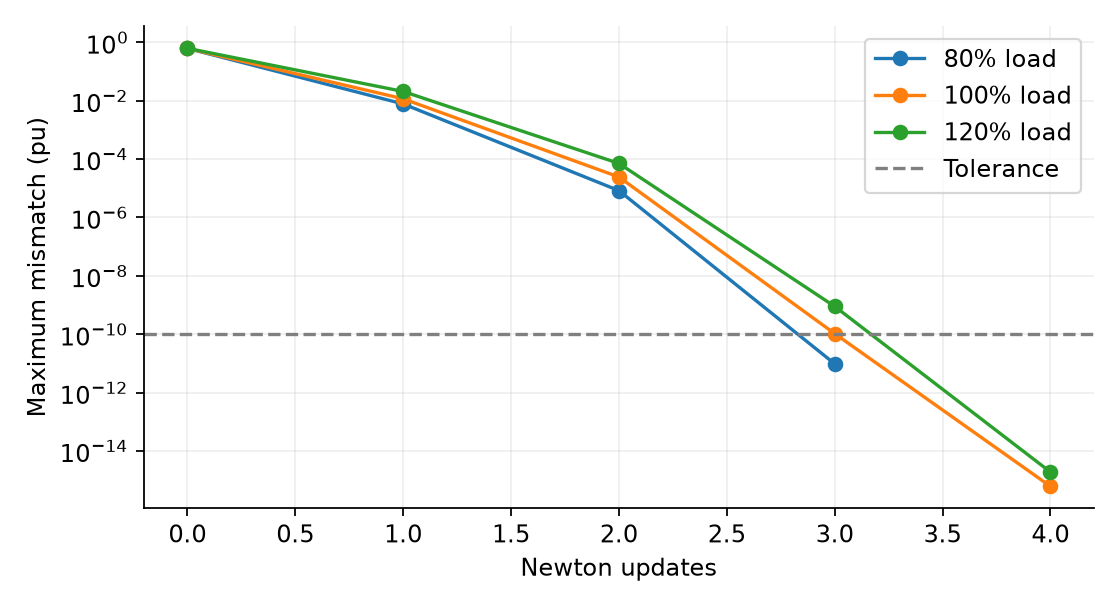
\includegraphics[width=0.7\textwidth]{../figures/3bus_convergence.png}
\caption{Quadratic convergence profile of the 3-bus test system.}
\label{fig:3bus_convergence}
\end{figure}

\subsection{Final Converged Operating State and Global Energy Conservation Audit}
The final converged state vector and branch power flows are summarized in Tables~\ref{tab:converged_bus} and~\ref{tab:converged_branch}.

\begin{table}[H]
\centering
\caption{Converged nodal electrical profile ($S_{\text{base}} = 100.0\text{ MVA}$).}
\label{tab:converged_bus}
\begin{tabular}{cccccccc}
\toprule
\textbf{Bus} & \textbf{Type} & \textbf{$U$ (p.u.)} & \textbf{$\delta$ (deg)} & \textbf{$P_G$ (MW)} & \textbf{$Q_G$ (Mvar)} & \textbf{$P_D$ (MW)} & \textbf{$Q_D$ (Mvar)} \\
\midrule
1 & Slack & 1.050000 & 0.000000 & 12.204690 & 77.807132 & 0.000 & 0.000 \\
2 & PV & 1.020000 & +1.024098 & 50.000000 & -46.193053 & 0.000 & 0.000 \\
3 & PQ & 0.984385 & -2.418330 & 0.000000 & 0.000000 & 60.000 & 25.000 \\
\midrule
\textbf{Total} & & & & \textbf{62.204690} & \textbf{31.614079} & \textbf{60.000} & \textbf{25.000} \\
\bottomrule
\end{tabular}
\end{table}

\begin{table}[H]
\centering
\caption{Converged directional branch power flows and transmission losses.}
\label{tab:converged_branch}
\begin{tabular}{cccccccc}
\toprule
\textbf{Line} & \textbf{From--To} & \textbf{$P_{ij}$ (MW)} & \textbf{$Q_{ij}$ (Mvar)} & \textbf{$P_{ji}$ (MW)} & \textbf{$Q_{ji}$ (Mvar)} & \textbf{$\Delta P_{ij}$ (MW)} & \textbf{$\Delta Q_{ij}$ (Mvar)} \\
\midrule
1 & 1--2 & -12.877333 & 57.077569 & 13.498408 & -55.214345 & 0.621075 & 1.863224 \\
2 & 1--3 & 25.082026 & 20.729563 & -24.313719 & -18.424643 & 0.768307 & 2.304920 \\
3 & 2--3 & 36.501592 & 9.021291 & -35.686281 & -6.575357 & 0.815311 & 2.445934 \\
\midrule
\textbf{Total} & & & & & & \textbf{2.204693} & \textbf{6.614078} \\
\bottomrule
\end{tabular}
\end{table}

\subsubsection{Global Energy Balance Check:}
\begin{align}
\sum P_{Gi} - \sum P_{Di} - \Delta P_{\Sigma} &= 62.204690 - 60.000000 - 2.204693 \nonumber \\
&= 2.204690 - 2.204693 = 0.000000\text{ MW} \quad (< 10^{-13}\text{ MW})
\end{align}
\begin{align}
\sum Q_{Gi} - \sum Q_{Di} - \Delta Q_{\Sigma} &= 31.614079 - 25.000000 - 6.614078 \nonumber \\
&= 6.614079 - 6.614078 = 0.000000\text{ Mvar} \quad (< 10^{-13}\text{ Mvar})
\end{align}
Global conservation of energy is strictly verified.

\section{Physical Operational Scenario Analysis}

\subsection{Scenario 1: System Load Scaling (80\% to 120\%)}
To investigate grid behavior under varying consumer load demand, the load at Bus 3 is scaled from 80\% ($48\text{ MW}, 20\text{ Mvar}$) to 120\% ($72\text{ MW}, 30\text{ Mvar}$). Table~\ref{tab:scenario1} summarizes the results.

\begin{table}[H]
\centering
\caption{Power flow response under system load scaling.}
\label{tab:scenario1}
\begin{tabular}{ccccccc}
\toprule
\textbf{Load Level} & \textbf{$P_D$ (MW)} & \textbf{$Q_D$ (Mvar)} & \textbf{$U_3$ (p.u.)} & \textbf{$\delta_3$ (deg)} & \textbf{$\Delta P_{\Sigma}$ (MW)} & \textbf{Iterations} \\
\midrule
80\% & 48.0 & 20.0 & 0.994686 & -1.670028 & 1.739606 & 3 \\
100\% (Base) & 60.0 & 25.0 & 0.984385 & -2.418330 & 2.204693 & 4 \\
120\% & 72.0 & 30.0 & 0.973711 & -3.183395 & 2.834110 & 4 \\
\bottomrule
\end{tabular}
\end{table}

\textbf{Physical Analysis:}
\begin{enumerate}
    \item \textbf{Longitudinal Voltage Drop:} As load increases from 80\% to 120\%, $U_3$ drops from $0.994686\text{ p.u.}$ to $0.973711\text{ p.u.}$, consistent with the transmission line voltage drop relation:
    \begin{equation}
    \Delta U \approx \frac{P R + Q X}{U}
    \end{equation}
    \item \textbf{Loss Growth:} Active losses increase from $1.739606\text{ MW}$ to $2.834110\text{ MW}$ (+62.9\% increase for a 40\% load step). This super-linear growth reflects the Joule heating relationship $\Delta P = I^2 R = \frac{P^2 + Q^2}{U^2} R$.
\end{enumerate}

\subsection{Scenario 2: Generator Terminal Voltage Regulation (PV Setpoint Tuning)}
The voltage setpoint $U_2$ at the PV generator bus is varied from $0.98\text{ p.u.}$ to $1.05\text{ p.u.}$, while maintaining active generation at $50.0\text{ MW}$. Table~\ref{tab:scenario2} presents the system response.

\begin{table}[H]
\centering
\caption{System response under PV generator terminal voltage regulation ($U_2$).}
\label{tab:scenario2}
\begin{tabular}{cccccc}
\toprule
\textbf{$U_2$ Setpoint (p.u.)} & \textbf{$U_3$ (p.u.)} & \textbf{$Q_{G2}$ (Mvar)} & \textbf{$Q_{G1}$ (Mvar)} & \textbf{$\Delta P_{\Sigma}$ (MW)} & \textbf{Iterations} \\
\midrule
0.980000 & 0.960154 & -118.127006 & +157.956391 & 4.943129 & 4 \\
1.000000 & 0.972284 & -82.958056 & +117.923624 & 3.321856 & 4 \\
1.020000 (Base) & 0.984385 & -46.193053 & +77.807132 & 2.204693 & 4 \\
1.050000 & 1.002482 & +11.958652 & +17.483475 & 1.480709 & 4 \\
\bottomrule
\end{tabular}
\end{table}

\textbf{Physical Analysis:}
\begin{enumerate}
    \item \textbf{$Q-U$ Sensitivity and Local Voltage Support:} Elevating $U_2$ from $0.98\text{ p.u.}$ to $1.05\text{ p.u.}$ raises the load bus voltage $U_3$ from $0.960154\text{ p.u.}$ to $1.002482\text{ p.u.}$, demonstrating how reactive power injection at PV buses provides voltage support to nearby load centers.
    \item \textbf{Reactive Power Shifting and Loss Reduction:} At $U_2 = 0.98\text{ p.u.}$, generator 2 underexcites severely ($Q_{G2} = -118.13\text{ Mvar}$), forcing the Slack generator to supply $157.96\text{ Mvar}$. This cross-network reactive power transfer increases branch currents and causes total active losses to rise to $4.943129\text{ MW}$. Raising $U_2$ to $1.05\text{ p.u.}$ allows Generator 2 to contribute $+11.96\text{ Mvar}$, reducing Slack reactive duty to $17.48\text{ Mvar}$ and reducing active losses to $1.480709\text{ MW}$ (a 70\% reduction in losses).
\end{enumerate}

\subsection{Scenario 3: Shunt Capacitive Compensation at Critical Load Bus}
To examine local reactive compensation at the load center, shunt capacitors providing $Q_C = 0.0, 10.0,$ and $20.0\text{ Mvar}$ are connected at Bus 3. Table~\ref{tab:scenario3} summarizes the results.

\begin{table}[H]
\centering
\caption{Impact of shunt capacitive compensation ($Q_C$) at load Bus 3.}
\label{tab:scenario3}
\begin{tabular}{ccccccc}
\toprule
\textbf{$Q_C$ (Mvar)} & \textbf{Net $Q_{D3}$ (Mvar)} & \textbf{$U_3$ (p.u.)} & \textbf{$\delta_3$ (deg)} & \textbf{$Q_{G1}$ (Mvar)} & \textbf{$\Delta P_{\Sigma}$ (MW)} & \textbf{Loss Reduction} \\
\midrule
0.0 (Base) & 25.0 & 0.984385 & -2.418330 & 77.807132 & 2.204693 & --- \\
10.0 & 15.0 & 0.995072 & -2.576658 & 73.245397 & 2.034843 & \textbf{-7.70\%} \\
20.0 & 5.0 & 1.005518 & -2.733153 & 68.767480 & 1.939748 & \textbf{-12.02\%} \\
\bottomrule
\end{tabular}
\end{table}

\textbf{Physical Analysis:}
Installing shunt capacitive compensation at Bus 3 produces three physical benefits:
\begin{enumerate}
    \item \textbf{Voltage Elevation:} $U_3$ rises from $0.984385\text{ p.u.}$ to $1.005518\text{ p.u.}$, restoring the voltage profile to nominal levels.
    \item \textbf{Reactive Current Relief:} Local capacitive generation supplies the inductive demand of the load, reducing upstream reactive power demand from the Slack generator ($Q_{G1}$ decreases from $77.81\text{ Mvar}$ to $68.77\text{ Mvar}$).
    \item \textbf{Transmission Loss Reduction:} Lower line current magnitudes reduce active power losses:
    \begin{equation}
    \Delta P_{ij} = \frac{P_{ij}^2 + (Q_{ij} - Q_C)^2}{U_j^2} \cdot r_{ij}
    \end{equation}
    Active power losses decrease by $12.02\%$ with $20\text{ Mvar}$ compensation.
\end{enumerate}

\subsection{Scenario 4: $N-1$ Transmission Line Outage Contingency Screening}
Transmission operators require that the network withstand the unplanned disconnection of any single line ($N-1$ criterion). Table~\ref{tab:scenario4} presents the post-contingency power flow results for all single line outages.

\begin{table}[H]
\centering
\caption{Post-contingency $N-1$ transmission line outage screening.}
\label{tab:scenario4}
\begin{tabular}{ccccccc}
\toprule
\textbf{Outaged Line} & \textbf{Status} & \textbf{$U_{\min}$ (p.u.)} & \textbf{Critical Bus} & \textbf{$\Delta P_{\Sigma}$ (MW)} & \textbf{Iters} & \textbf{Security Assessment} \\
\midrule
\textbf{None (Base)} & Converged & 0.984385 & Bus 3 & 2.204693 & 4 & \textbf{Compliant (Secure)} \\
\textbf{Line 1--2} & Converged & 0.983620 & Bus 3 & 2.022847 & 4 & \textbf{Compliant (Secure)} \\
\textbf{Line 1--3} & Converged & 0.927755 & Bus 3 & 3.396328 & 4 & \textbf{Violation ($U < 0.95$)} \\
\textbf{Line 2--3} & Converged & 0.924591 & Bus 3 & 5.277141 & 4 & \textbf{Severe Violation ($U < 0.95$)} \\
\bottomrule
\end{tabular}
\end{table}

\textbf{Physical Analysis:}
\begin{enumerate}
    \item \textbf{Transition from Meshed Loop to Radial Topology:} Outage of Line 1--3 or Line 2--3 eliminates the parallel feeding path to load Bus 3. Power that previously flowed through two parallel corridors is forced through a single remaining corridor.
    \item \textbf{Voltage Depression:} With Line 2--3 outaged, all $60\text{ MW}$ and $25\text{ Mvar}$ consumed at Bus 3 must be supplied via Line 1--3 ($z_{13} = 0.08 + j0.24\text{ p.u.}$). The heavy line loading causes $U_3$ to collapse to $0.924591\text{ p.u.}$, violating statutory grid limits ($U \ge 0.95\text{ p.u.}$) and requiring operator intervention (e.g., reactive compensation or load shedding).
    \item \textbf{Loss Increase:} With Line 2--3 out of service, active losses increase to $5.277141\text{ MW}$ (+139.4\% increase relative to base case), reflecting heavy loading on the remaining transmission corridor.
\end{enumerate}

% ----------------------------------------------------
% CHAPTER 5: CONCLUSION & ENGINEERING INSIGHTS
% ----------------------------------------------------
\chapter{Conclusion \& Engineering Insights}

\section{Summary of Analytical and Numerical Achievements}
This Project I study has established a mathematically transparent, white-box investigation of the steady-state AC power flow problem utilizing the Polar Newton--Raphson method. The key contributions include:
\begin{enumerate}
    \item \textbf{Rigorous Mathematical Formulation:} Established the exact non-linear AC polar power equations and derived analytical closed-form partial derivatives for all eight cases of the partitioned Jacobian matrix ($\mathbf{H}, \mathbf{N}, \mathbf{M}, \mathbf{L}$), eliminating finite-difference approximations.
    \item \textbf{Step-by-Step Manual Numerical Benchmark:} Completed an exhaustive manual calculation for Iteration 1 on the benchmark 3-bus transmission network, detailing every primitive admittance, matrix assembly, power mismatch, Jacobian derivative, and linear solve.
    \item \textbf{Machine-Precision Cross-Validation:} Demonstrated 1:1 numerical agreement between manual derivations and the developed solver down to IEEE-754 double precision ($< 10^{-16}\text{ p.u.}$ discrepancy), confirmed quadratic convergence down to $\Vert \mathbf{f} \Vert_\infty \le 10^{-10}\text{ p.u.}$ across 4 iterations, and verified global system active and reactive power balance.
    \item \textbf{Operational Grid Insights:} Analyzed network responses across four realistic operating conditions: load scaling, generator terminal voltage regulation, shunt capacitive compensation, and $N-1$ line outage contingencies.
\end{enumerate}

\section{Key Physical Insights into AC Power Flow Dynamics}
\begin{enumerate}
    \item \textbf{Quadratic Convergence Characteristics:} When initialized close to the solution (such as via standard flat start), the Newton--Raphson method demonstrates quadratic convergence ($\Vert \mathbf{f}^{(m+1)} \Vert \le C \Vert \mathbf{f}^{(m)} \Vert^2$), driving mismatches from $0.619\text{ p.u.}$ to $6.1 \times 10^{-16}\text{ p.u.}$ in 4 iterations.
    \item \textbf{Physical Decoupling Properties in High-Voltage Grids:} In high-voltage transmission networks with high $X/R$ ratios ($x_{ij} \gg r_{ij}$), the Jacobian exhibits physical decoupling:
    \begin{itemize}
        \item Block $\mathbf{H}$ ($\partial \mathbf{P} / \partial \boldsymbol{\delta}$) and Block $\mathbf{L}$ ($\partial \mathbf{Q} / \partial \mathbf{U}$) contain large dominant entries.
        \item Block $\mathbf{N}$ ($\partial \mathbf{P} / \partial \mathbf{U}$) and Block $\mathbf{M}$ ($\partial \mathbf{Q} / \partial \boldsymbol{\delta}$) are weak, reflecting the strong $P-\delta$ and $Q-U$ decoupling inherent to high-voltage transmission grids.
    \end{itemize}
    \item \textbf{Impact of Reactive Compensation on Grid Security:} Shunt capacitor compensation at load buses provides local reactive power, elevates terminal voltages, reduces upstream transmission line currents, and lowers system active power losses.
\end{enumerate}

\section{Limitations of Polar Newton--Raphson and Advanced Future Research Directions}
While this project provides a rigorous foundation in AC power flow computing, several technical extensions remain valuable for future exploration:
\begin{enumerate}
    \item \textbf{Fast Decoupled Power Flow (FDPF):} Exploiting the $P-\delta$ and $Q-U$ decoupling properties by holding the $B'$ and $B''$ sub-matrices constant, eliminating the need to update and factorize the Jacobian matrix at every iteration.
    \item \textbf{Sparse Matrix Factorization for Large-Scale Grids:} Implementing Sparse LU factorization with AMD (Approximate Minimum Degree) ordering to handle large IEEE test systems (e.g., 14-bus, 30-bus, 118-bus) with $O(N)$ computational complexity.
    \item \textbf{Automatic PV-to-PQ Switching:} Implementing automatic generator reactive power capability limit enforcement during iteration.
    \item \textbf{Optimal Power Flow (OPF):} Integrating the power flow equality constraints into optimization algorithms to minimize fuel costs, transmission losses, or generation curtailment.
\end{enumerate}

% ==================== REFERENCES ====================
\begin{thebibliography}{99}
\addcontentsline{toc}{chapter}{References}

\bibitem{Grainger1994}
J.~J.~Grainger and W.~D.~Stevenson, \textit{Power System Analysis}, McGraw-Hill, New York, NY, USA, 1994.

\bibitem{Kundur1994}
P.~Kundur, \textit{Power System Stability and Control}, McGraw-Hill, New York, NY, USA, 1994.

\bibitem{Glover2016}
J.~D.~Glover, M.~S.~Sarma, and T.~Overbye, \textit{Power System Analysis and Design}, 6th ed., Cengage Learning, Boston, MA, USA, 2016.

\bibitem{Wood2013}
A.~J.~Wood, B.~F.~Wollenberg, and G.~B.~Sheblé, \textit{Power Generation, Operation, and Control}, 3rd ed., John Wiley \& Sons, Hoboken, NJ, USA, 2013.

\bibitem{Tinney1967}
W.~F.~Tinney and C.~E.~Hart, ``Power flow solution by Newton's method,'' \textit{IEEE Transactions on Power Apparatus and Systems}, vol.~PAS-86, no.~11, pp.~1449--1460, Nov. 1967.

\bibitem{Stott1974}
B.~Stott and O.~Alsac, ``Fast decoupled load flow,'' \textit{IEEE Transactions on Power Apparatus and Systems}, vol.~PAS-93, no.~3, pp.~859--869, May 1974.

\bibitem{HUST_EE3810E}
Department of Power Systems, \textit{Course Syllabus and Project Guidelines: Project I (EE3810E)}, School of Electrical and Electronic Engineering, Hanoi University of Science and Technology, 2024.

\bibitem{EVN_GridCode}
Ministry of Industry and Trade (MOIT), \textit{Circular No. 25/2016/TT-BCT: Regulations on National Electric Power Transmission System (Vietnam Transmission Grid Code)}, Hanoi, Vietnam, 2016.

\end{thebibliography}

\end{document}
